
\section{Experiments}
In this section, the details of training road embeddings by the next-hop prediction model will be given. And we will explain the process of parameter tuning. A verification for the functionality of road correlation, as well as an analysis and visualization are also stated in this section.

\subsection{Settings}
Our experiments were performed on a sever equipped with Intel(R) Xeon(R) Silver 4216 CPU @ 2.10GHz and an NVIDIA GeForce RTX 2080Ti graphics card. The PyTorch\cite{pytorch} version is 1.7.1 with Python 3.7.11.

\begin{table}[htb]
    \begin{center}
        \caption{Tuned parameters for next-hop prediction.}
        \label{next-hop_params}
        \begin{tabular}{clll}
            \toprule
  
            \textbf{Notation} & \textbf{Parameter} & \textbf{Search Space} & \textbf{Selected Value}\\
  
            \midrule
  
            $w$ & Window size & $\{5 \}$ & $5$\\
            $p$ & Sampling proportion & $\{0.05, 0.1, 0.2, 0.4, 0.8\}$ & $0.8$\\
            $d_r$ & Road embedding dimension & $\{16, 32, 64, 128 \}$ & $64$\\
            $d_h$ & LSTM hidden size & $\{32, 64, 128, 256 \}$ & $256$\\
            $d_o$ & Linear output dimension & $d_o=n_r=\#roads$ & $492$\\
            ~ & Batch size & $\{64, 128, 256, 512 \}$ & $256$\\
            ~ & Learning rate & $\{0.0001, 0.001\}$ & $0.0001$\\
            ~ & Early stopping epochs & $\{5, 10, 15\}$ & $10$\\
  
            \bottomrule
        \end{tabular}
    \end{center}
\end{table}

For the next-hop prediction model, the window size for trajectory fragments generation was set as $w=5$. After data processing, we got 1,751,602 trajectories in total. Removing too long and too short ones, there were 1,351,700 remaining. Then we put the trajectories into 24 bins according to their starting time and randomly sampled $p=80\%$ data in each bin to combine as the whole dataset. Finally, there were 1,076,886 trajectories. The data ratio for training, validation, and testing was set as 7:1:2. After window sliding, we got 10,228,578 trajectory fragments for training, and 1,455,100 for validation. Adam\cite{adam} algorithm was employed to control the overall training process, and the loss function was \textit{Cross Entropy Loss}. The complete parameter selection is given in table \ref{next-hop_params}.

For traffic state prediction models, the experiments were performed on DL-Traff\cite{dl-traff}, an open-source benchmark platform. As for the parameters, the input steps and prediction steps were both set to 12. The size of traffic state matrix is $n_r\times n_t=492\times 8064$. The data split ratio was also 7:1:2, and after sampling, we got 6437 traffic state vectors for training. The optimizer was Adam where the learning rate was set as 0.001, and the loss function was \textit{Mean Squared Error (MSE) Loss}. Batch size was set to 32 in order to avoid the \textit{CUDA Out of Memory} exception. Similarly, the training process would be early-stopped if the validation loss was not decreasing for 10 epochs, then the best model on validation data would be saved. Details are provided in table \ref{traff_pred_params}.

\begin{table}[htb]
    \begin{center}
        \caption{Parameters for traffic state prediction.}
        \label{traff_pred_params}
        \begin{tabular}{cll}
            \toprule
  
            \textbf{Notation} & \textbf{Parameter} & \textbf{Value}\\
  
            \midrule
  
            $w_{in}$ & Input steps & $12$\\
            $w_{out}$ & Prediction steps & $12$\\
            ~ & Batch size & $32$\\
            ~ & Learning rate & $0.001$\\
            ~ & Early stopping epochs & $10$\\
            ~ & Max training epochs & $200$\\
  
            \bottomrule
        \end{tabular}
    \end{center}
\end{table}

\subsection{Baseline Models}
We selected two baseline traffic prediction models that can effectively capture the spatial dependencies in the graph.

\begin{itemize}
    \item \textbf{STGCN}\cite{STGCN} (Spatio-Temporal Graph Convolutional Networks). STGCN is proposed in 2018, which is one of the earliest GCN models for traffic prediction. It uses gated TCN\cite{TCN} to capture temporal dependencies and applies spectral graph convolution\cite{GCN0} on graph to model the spatial dependencies.
    \item \textbf{DCRNN}\cite{DCRNN} (Diffusion Convolutional Recurrent Neural Network). DCRNN is another typical GCN model that is also proposed in 2018. Instead of spectral graph convolution, it implements diffusion convolution through bidirectional random walk to capture the transition information. Temporally, it integrates diffusion convolution into GRU and proposed an encoder-decoder structure to enable multistep prediction.
\end{itemize}

We set the input graph as (1) \textit{adjacency matrix} $A$, (2) \textit{refined adjacency matrix} $A'$ to compare their performance and illustrate the effect of road correlation in traffic state prediction. The corresponding models are denoted as STGCN-$A$, STGCN-$A'$, DCRNN-$A$ and DCRNN-$A'$. In addition, we kept the (3) \textit{road correlation matrix} $C$ as input to give an ablation experiment. They are denoted as STGCN-$C$ and DCRNN-$C$.

\subsection{Evaluation Metrics}
Following previous studies, we use \textit{Root Mean Square Error (RMSE)}, \textit{Mean Absolute Error (MAE)}, and \textit{Mean Absolute Percentage Error (MAPE)} as the metrics to show the performance of different methods. Zero values will be ignored, and lower errors indicate better performance. The definition of them are as following.

\begin{equation}
    \begin{aligned}
        MAE&=\frac 1n\sum_{i=1}^n|\hat{y_i}-y_i|\\
        MAPE&=\frac 1n\sum_{i=1}^n|\frac{\hat{y_i}-y_i}{y_i}|\\
        RMSE&=\sqrt{\frac 1n\sum_{i=1}^n(\hat{y_i}-y_i)^2}
    \end{aligned}
\end{equation}

\begin{table}[t!]
    \renewcommand\arraystretch{1.2} % line space
    \begin{center}
        \caption{Performance evaluation results.}
        \label{performance_results}
        \resizebox{\textwidth}{!}{
            \begin{tabular}{c|c|c|ccc|ccc|ccc}
                \toprule
                
                \multirow{2}{*}{Traffic State} & \multirow{2}{*}{Model} & \multirow{2}{*}{G Type} & \multicolumn{3}{c|}{3 Steps / 15 min} & \multicolumn{3}{c|}{6 Steps / 30 min} & \multicolumn{3}{c}{12 Steps / 60 min} \\

                \cline{4-12}

                                                 &                        &                         & RMSE       & MAE       & MAPE        & RMSE      & MAE       & MAPE        & RMSE       & MAE        & MAPE        \\
                \hline

                \multirow{23}{*}{Flow}           & HA                     & -                       & 5.84       & 4.35      & 41.18\%     & 5.82      & 4.34      & 41.10\%     & 5.8        & 4.33       & 40.98\%     \\
                                                 & CP                     & -                       & 7.23       & 5.37      & 50.13\%     & 7.23      & 5.38      & 50.15\%     & 7.24       & 5.38       & 50.16\%     \\
                \cline{2-12}
                                                 & \multirow{7}{*}{STGCN} & A                       & 4.44       & 3.46      & 33.00\%     & 4.64      & 3.57      & 33.64\%     & 5.07       & 3.88       & 36.07\%     \\
                                                 &                        & OD                      & 4.42       & 3.44      & 33.08\%     & 4.72      & 3.61      & 33.73\%     & 5.43       & 4.12       & 37.90\%     \\
                                                 &                        & P                       & 5.43       & 4.08      & 37.40\%     & 5.74      & 4.39      & 40.47\%     & 6.35       & 4.75       & 45.24\%     \\
                                                 &                        & COS                     & 5.43       & 4.08      & 37.40\%     & 5.74      & 4.39      & 40.47\%     & 6.35       & 4.75       & 45.24\%     \\
                                                 &                        & DTW                     & 4.39       & 3.4       & 32.40\%     & 4.63      & 3.57      & 33.70\%     & 5.03       & 3.82       & 35.73\%     \\
                                                 &                        & C                       & 4.38       & 3.4       & 32.41\%     & 4.56      & 3.52      & 33.33\%     & 5.03       & 3.82       & 35.87\%     \\
                                                 &                        & A'                      & 4.42       & 3.43      & 32.67\%     & 4.61      & 3.55      & 33.35\%     & 5.03       & 3.82       & 35.80\%     \\
                \cline{2-12}
                                                 & \multirow{7}{*}{DCRNN} & A                       & 4.47       & 3.46      & 33.01\%     & 4.66      & 3.6       & 34.06\%     & 5.03       & 3.85       & 35.76\%     \\
                                                 &                        & OD                      & 4.49       & 3.46      & 32.92\%     & 4.71      & 3.61      & 34.16\%     & 5.15       & 3.87       & 36.19\%     \\
                                                 &                        & P                       & 7.13       & 5.55      & 50.66\%     & 6.86      & 5.3       & 48.81\%     & 7.97       & 6.05       & 55.66\%     \\
                                                 &                        & COS                     & 4.42       & 3.42      & 32.71\%     & 4.6       & 3.53      & 33.46\%     & 5.01       & 3.79       & 35.35\%     \\
                                                 &                        & DTW                     & 11.11      & 8.83      & 76.44\%     & 11.9      & 9.9       & 89.60\%     & 12.56      & 10.58      & 97.62\%     \\
                                                 &                        & C                       & 8.19       & 6.13      & 55.66\%     & 8.18      & 6.13      & 55.64\%     & 8.13       & 6.09       & 55.33\%     \\
                                                 &                        & A'                      & 4.23       & 3.28      & 31.46\%     & 4.63      & 3.54      & 33.60\%     & 4.98       & 3.77       & 35.26\%     \\
                \cline{2-12}
                                                 & \multirow{7}{*}{GWNET} & A                       & 4.45       & 3.45      & 32.66\%     & 4.69      & 3.61      & 33.97\%     & 5.21       & 3.94       & 36.46\%     \\
                                                 &                        & OD                      & 4.51       & 3.48      & 32.76\%     & 4.78      & 3.65      & 34.04\%     & 5.45       & 4.07       & 36.81\%     \\
                                                 &                        & P                       & 4.31       & 3.34      & 32.00\%     & 4.58      & 3.51      & 33.44\%     & 4.93       & 3.73       & 34.93\%     \\
                                                 &                        & COS                     & 4.48       & 3.47      & 33.12\%     & 4.86      & 3.72      & 34.94\%     & 5.48       & 4.12       & 37.78\%     \\
                                                 &                        & DTW                     & 4.61       & 3.54      & 33.30\%     & 5.06      & 3.82      & 35.41\%     & 5.72       & 4.22       & 38.26\%     \\
                                                 &                        & C                       & 4.48       & 3.45      & 32.82\%     & 4.68      & 3.58      & 33.79\%     & 5.13       & 3.85       & 35.71\%     \\
                                                 &                        & A'                      & 4.41       & 3.41      & 32.61\%     & 4.57      & 3.51      & 33.31\%     & 4.98       & 3.76       & 35.25\%     \\
                \hline
                \hline

                \multirow{23}{*}{Speed}          & HA                     & -                       & 7.33       & 5.28      & 26.07\%     & 7.33      & 5.28      & 26.08\%     & 7.32       & 5.27       & 26.04\%     \\
                                                 & CP                     & -                       & 9.3        & 6.5       & 30.65\%     & 9.3       & 6.51      & 30.66\%     & 9.3        & 6.51       & 30.63\%     \\
                \cline{2-12}
                                                 & \multirow{7}{*}{STGCN} & A                       & 6.6        & 4.65      & 23.67\%     & 6.63      & 4.66      & 24.22\%     & 6.71       & 4.74       & 24.01\%     \\
                                                 &                        & OD                      & 6.61       & 4.66      & 23.64\%     & 6.62      & 4.67      & 24.05\%     & 6.71       & 4.76       & 24.14\%     \\
                                                 &                        & P                       & 6.6        & 4.64      & 23.61\%     & 7.28      & 5.36      & 27.06\%     & 6.5        & 4.56       & 24.30\%     \\
                                                 &                        & COS                     & 6.6        & 4.64      & 23.61\%     & 7.28      & 5.36      & 27.06\%     & 6.68       & 4.72       & 23.95\%     \\
                                                 &                        & DTW                     & 6.94       & 4.99      & 26.26\%     & 7.16      & 5.21      & 27.13\%     & 6.98       & 5.03       & 25.96\%     \\
                                                 &                        & C                       & 6.62       & 4.66      & 23.87\%     & 6.63      & 4.69      & 24.10\%     & 6.67       & 4.71       & 24.04\%     \\
                                                 &                        & A'                      & 6.6        & 4.65      & 23.66\%     & 6.63      & 4.68      & 24.04\%     & 6.67       & 4.72       & 24.00\%     \\
                \cline{2-12}
                                                 & \multirow{7}{*}{DCRNN} & A                       & 6.61       & 4.65      & 23.82\%     & 6.65      & 4.69      & 24.00\%     & 6.71       & 4.76       & 24.29\%     \\
                                                 &                        & OD                      & 6.83       & 4.87      & 25.04\%     & 7.02      & 5.07      & 25.37\%     & 7.3        & 5.33       & 26.64\%     \\
                                                 &                        & P                       & 6.59       & 4.64      & 23.80\%     & 6.63      & 4.67      & 23.95\%     & 6.67       & 4.73       & 24.17\%     \\
                                                 &                        & COS                     & 6.7        & 4.75      & 24.63\%     & 6.79      & 4.85      & 25.13\%     & 6.98       & 5.04       & 25.61\%     \\
                                                 &                        & DTW                     & 6.63       & 4.65      & 23.95\%     & 6.67      & 4.7       & 24.12\%     & 6.74       & 4.8        & 24.41\%     \\
                                                 &                        & C                       & 8.41       & 6.39      & 30.90\%     & 8.45      & 6.42      & 31.13\%     & 8.46       & 6.43       & 31.18\%     \\
                                                 &                        & A'                      & 6.62       & 4.65      & 23.82\%     & 6.66      & 4.68      & 23.99\%     & 6.71       & 4.75       & 24.25\%     \\
                \cline{2-12}
                                                 & \multirow{7}{*}{GWNET} & A                       & 6.84       & 4.84      & 25.51\%     & 7.06      & 5.06      & 27.07\%     & 7.88       & 5.82       & 31.48\%     \\
                                                 &                        & OD                      & 6.61       & 4.64      & 23.83\%     & 6.65      & 4.68      & 24.07\%     & 6.71       & 4.76       & 24.45\%     \\
                                                 &                        & P                       & 7.03       & 5.05      & 26.91\%     & 7.1       & 5.16      & 26.62\%     & 7.37       & 5.4        & 27.61\%     \\
                                                 &                        & COS                     & 6.62       & 4.65      & 23.85\%     & 6.66      & 4.69      & 24.15\%     & 6.74       & 4.78       & 24.75\%     \\
                                                 &                        & DTW                     & 6.62       & 4.66      & 23.82\%     & 6.66      & 4.7       & 24.06\%     & 6.72       & 4.77       & 24.52\%     \\
                                                 &                        & C                       & 6.62       & 4.67      & 23.65\%     & 6.65      & 4.7       & 23.77\%     & 6.71       & 4.78       & 24.00\%     \\
                                                 &                        & A'                      & 6.59       & 4.64      & 23.46\%     & 6.63      & 4.68      & 23.56\%     & 6.69       & 4.74       & 23.85\%     \\
                \bottomrule
            \end{tabular}
        }
    \end{center}
\end{table}

\subsection{Performance and Analysis}
First, we introduce the performance of the next-hop prediction model. We tried tens of parameter combinations and finally reached $5.47$ on test loss and $73.47\%$ on prediction accuracy. The embedding matrix $E$ in the model was saved for the computation of \textit{refined adjacency matrix} $A'$. Then the comparison of the traffic state prediction models' performance are given in table \ref{performance_results}. To demonstrate how the prediction accuracy varies with time, we report the metrics for 15, 30, 60-minutes ahead prediction. From the table, we obtain the following observations:

\begin{itemize}
    \item Our $A'$-version has the smallest error in almost every step for the three metrics, especially \textit{MAPE}. This illustrates that the proposed \textit{trajectory-based road correlation} can better capture the spatial dependencies on the road network graph than the adjacency matrix which cannot reflect the real world traffic scenarios.
    \item With the increasing of prediction steps, all models tend to perform worse because of the difficulty in long-range prediction. Coincidentally, the improvement of long-range metrics is also smaller than short-range. Compared to original $A$-version, our $A'$-version performs best in short-range prediction. For example, for 15-minutes ahead prediction, DCRNN-$A'$ has a $1.55\%$ lower \textit{MAPE} than DCRNN-$A$. But when turning to 60-minutes ahead, the improvement decreases to $0.5\%$. We think this is caused by the limitation of the next-hop model. In the last section, we mentioned that LSTM can capture high-order dependency. However, it is still incapable to catch the dependency for a 60-minutes duration. What's more, our choice for the window size $w=5$ may also lead to the short-sight of LSTM.
    \item STGCN is good at predicting traffic speed, while DCRNN is expert in traffic flow prediction. However, the difference between them in speed prediction is not as large as flow. The reason is that our \textit{trajectory-based road correlation} captures the road transition information, which is directly related to the propagation of traffic flow, but have nothing to do with the variation of traffic speed.
    \item \textbf{Ablation Experiment.} Our aim is to check the contribution of adjacency matrix refinement to the final performance. For the ablation study, we build the models STGCN-$C$ and DCRNN-$C$ that directly take correlation matrix $C$ as input. For STGCN, the results show that the $A'$-version is better in almost all cases. But what we want to emphasize is that the refinement process is essential for DCRNN. The table shows that DCRNN-$C$ performs very bad, such as the $55\%$ \textit{MAPE} for traffic flow prediction. In addition, when training the model, we found that the training loss is always increasing, i.e. the model cannot converge. This indicates that the diffusion convolution can only take binary relations as input. Therefore, it is necessary to use \textit{refined adjacency matrix} as DCRNN's input.
\end{itemize}

\subsection{Parameter Study}
\begin{figure}[htb]
    \centering
    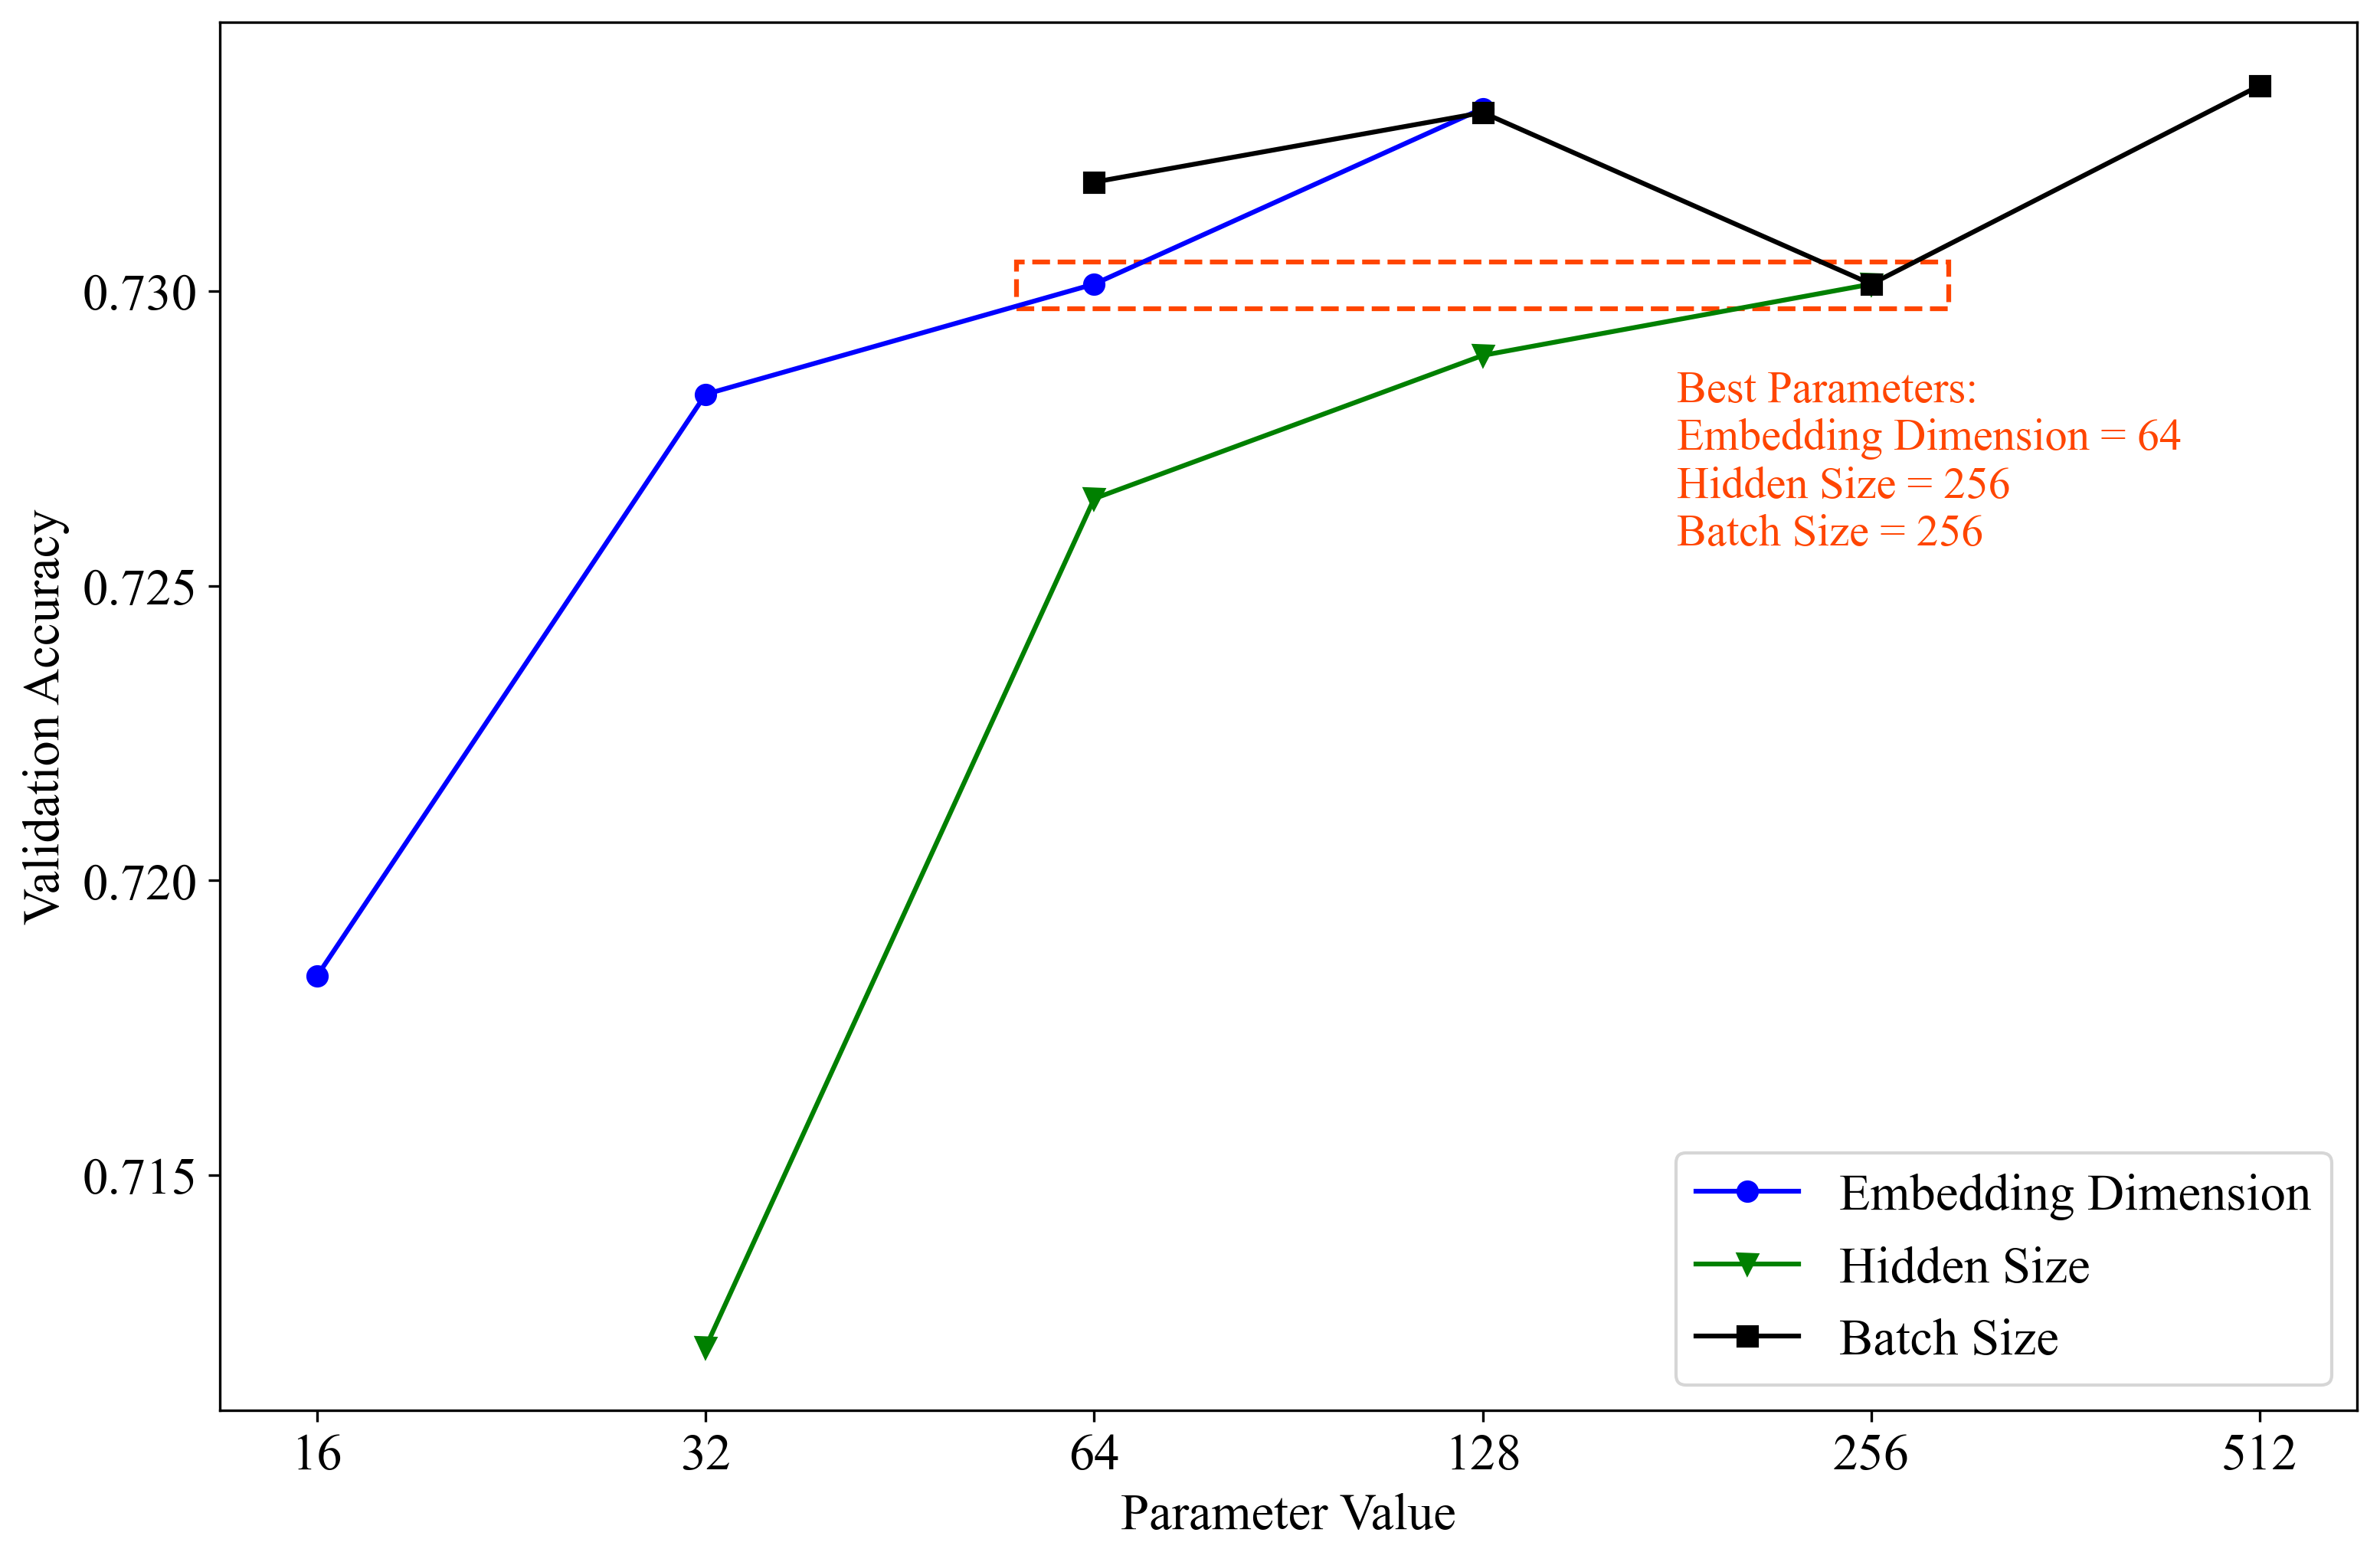
\includegraphics[width=\textwidth]{images/next-hop_param.png}
    \caption{Parameter tuning for the next-hop prediction model.}
    \label{fig: next-hop_param}
\end{figure}

This section introduces parameter analysis to provide a closer insight into our models. At first, the parameter tuning process of the next-hop prediction model is given in figure \ref{fig: next-hop_param}, including the choices for road embedding dimension, LSTM hidden size and batch size. The parameter search candidates are given in the above table \ref{next-hop_params} in section 6.1. Actually, according to the table, tuning these three parameters needs to search $4^3=64$ combinations, and should be plotted in a 3-D chart. But for the convenience of drawing, we set other two parameters fixed when studying one of them. The figure shows the variation of the prediction accuracy on validation dataset with parameter values. From it, we observe that (1) the prediction accuracy is positively related to embedding dimension and LSTM hidden size, because they become more representative. (2) Batch size has no clearly positive or negative relation with accuracy, needing case-to-case analysis. (3) Large embedding dimension and LSTM hidden size combinations will lead to lower accuracy, which is not displayed in the figure. Nevertheless, it is still necessary to be emphasized. Finally, considering the overall performance and the ability of generalization, we choose the parameters shown in the orange rectangle with $73.01\%$ prediction accuracy.

\begin{figure}[htb]
    \centering
    \caption{Variation of STGCN-$A'$ prediction \textit{MAPE} with $k$.}
    \label{fig: k}
    \begin{subfigure}[t]{0.49\linewidth}
        \centering
        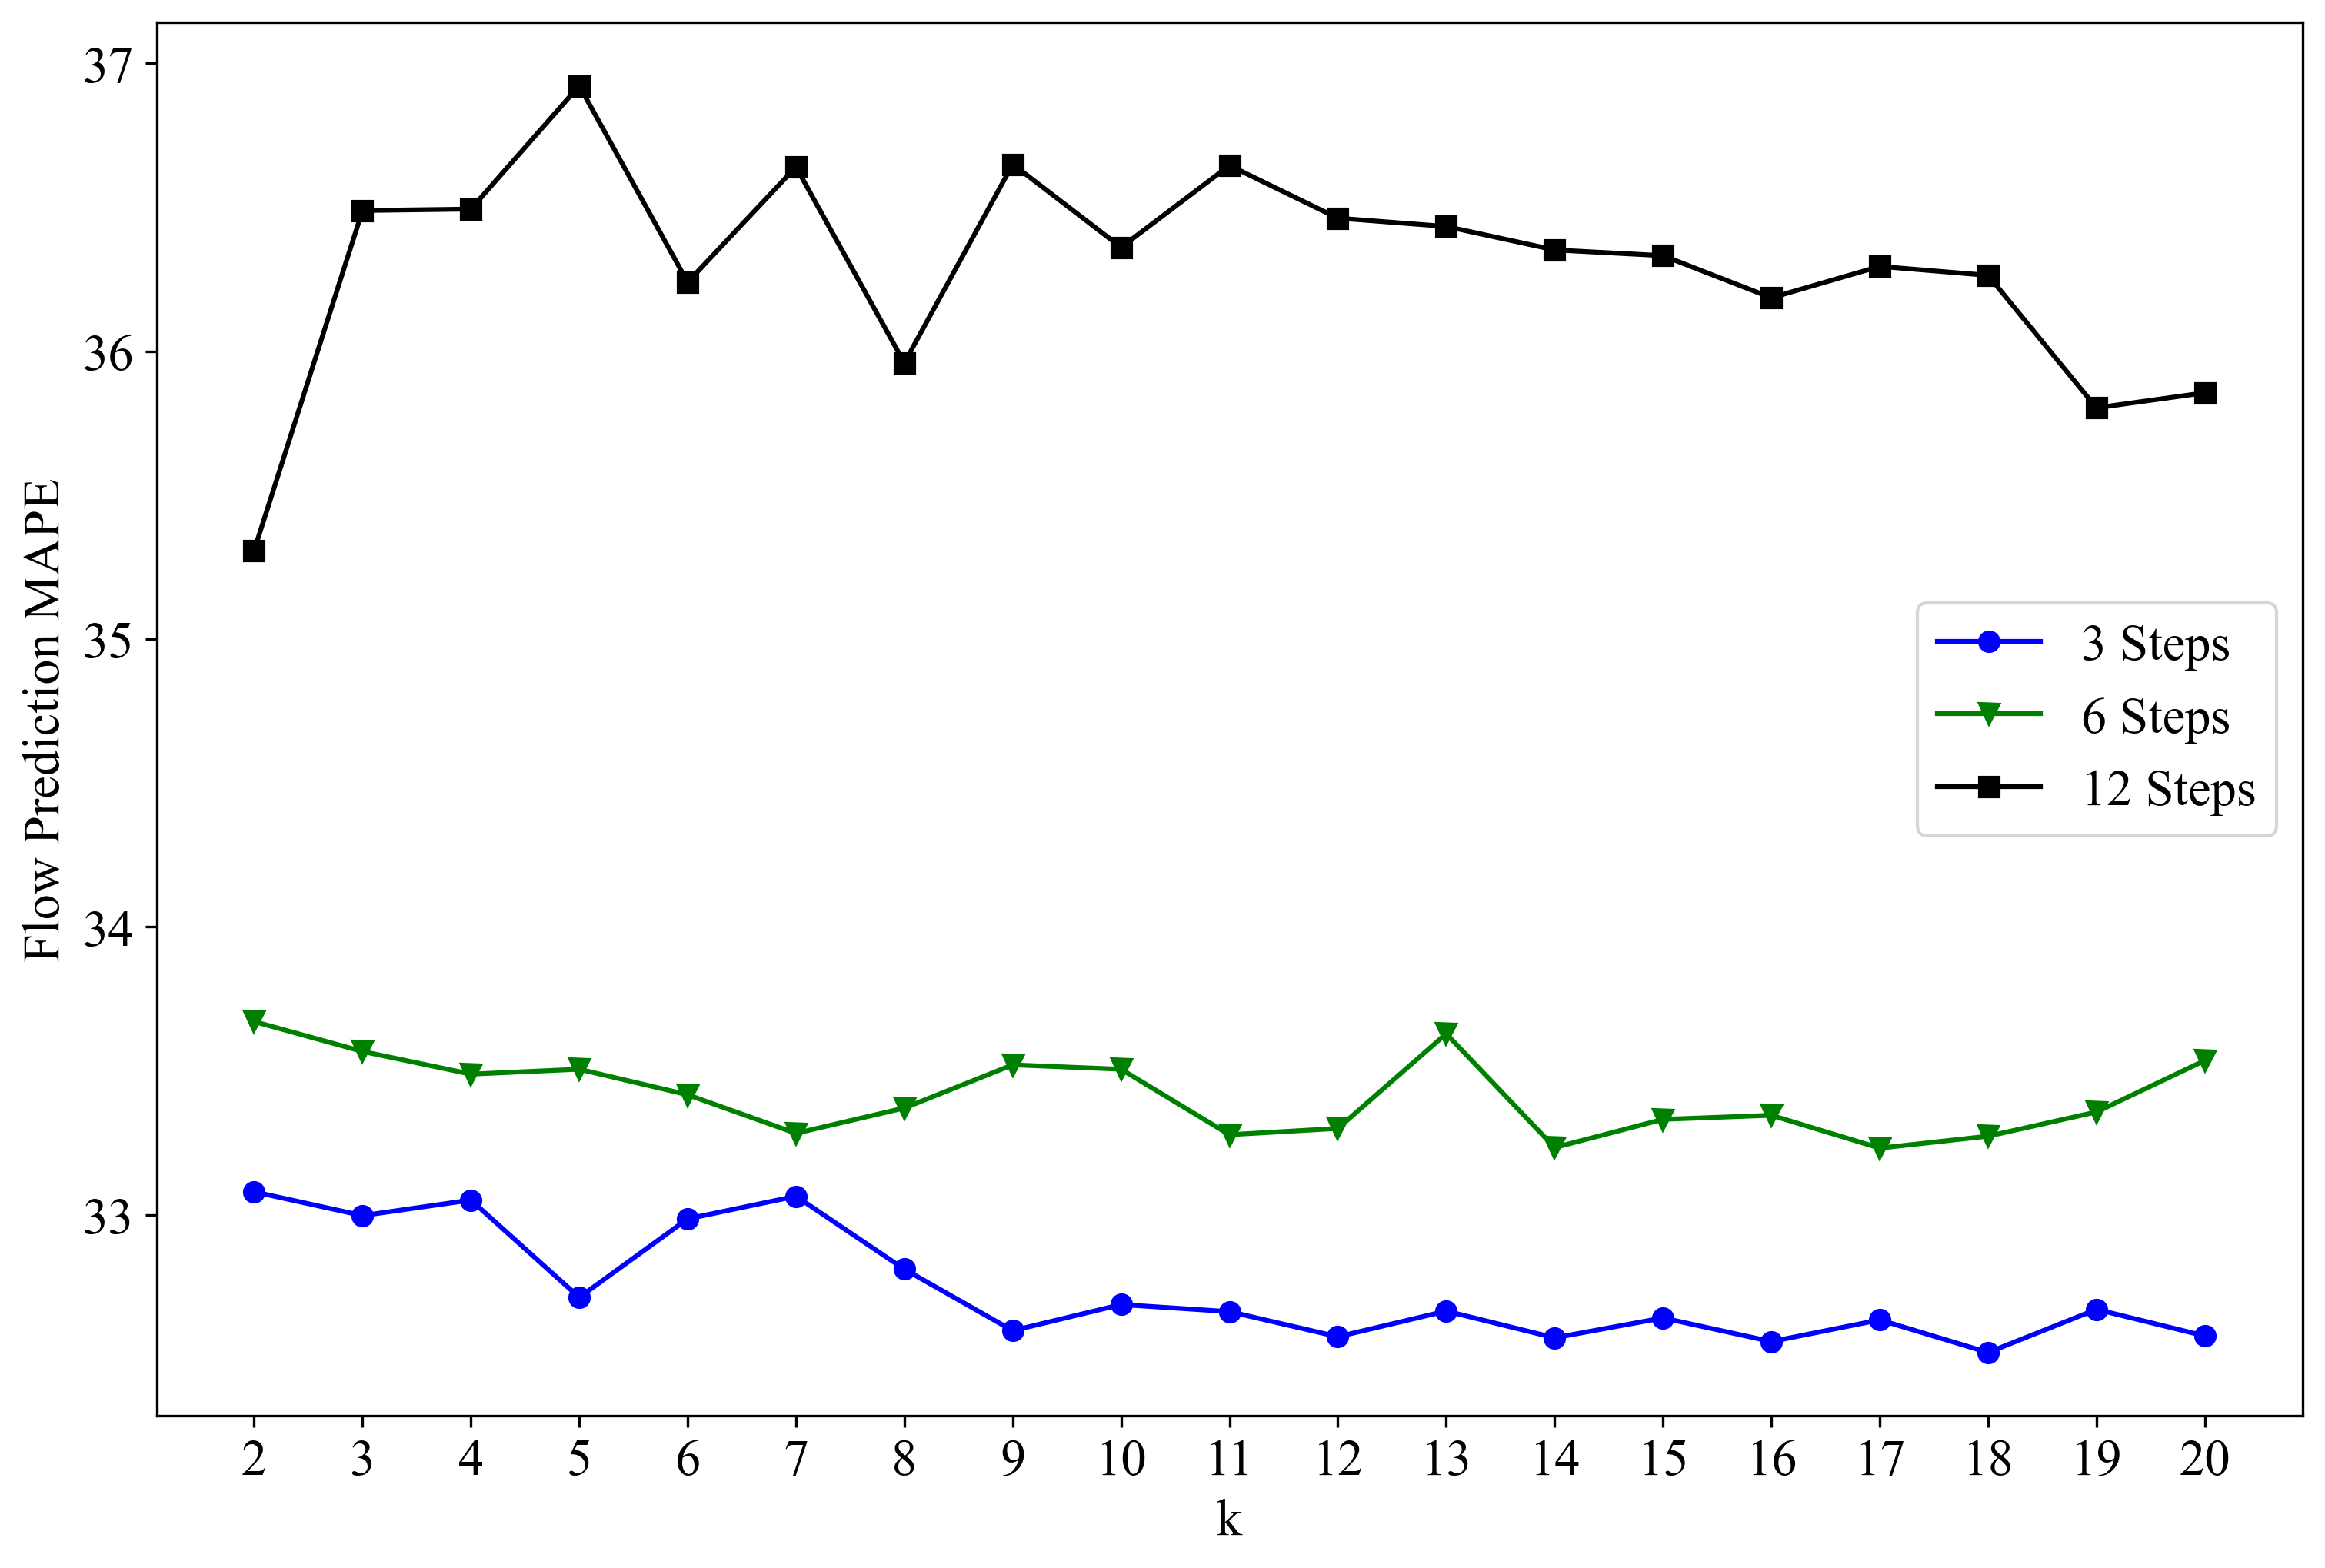
\includegraphics[width=\textwidth]{images/k-flow.png}
        \caption{Traffic flow prediction}
        \label{fig: k-flow}
    \end{subfigure}
    \begin{subfigure}[t]{0.49\linewidth}
        \centering
        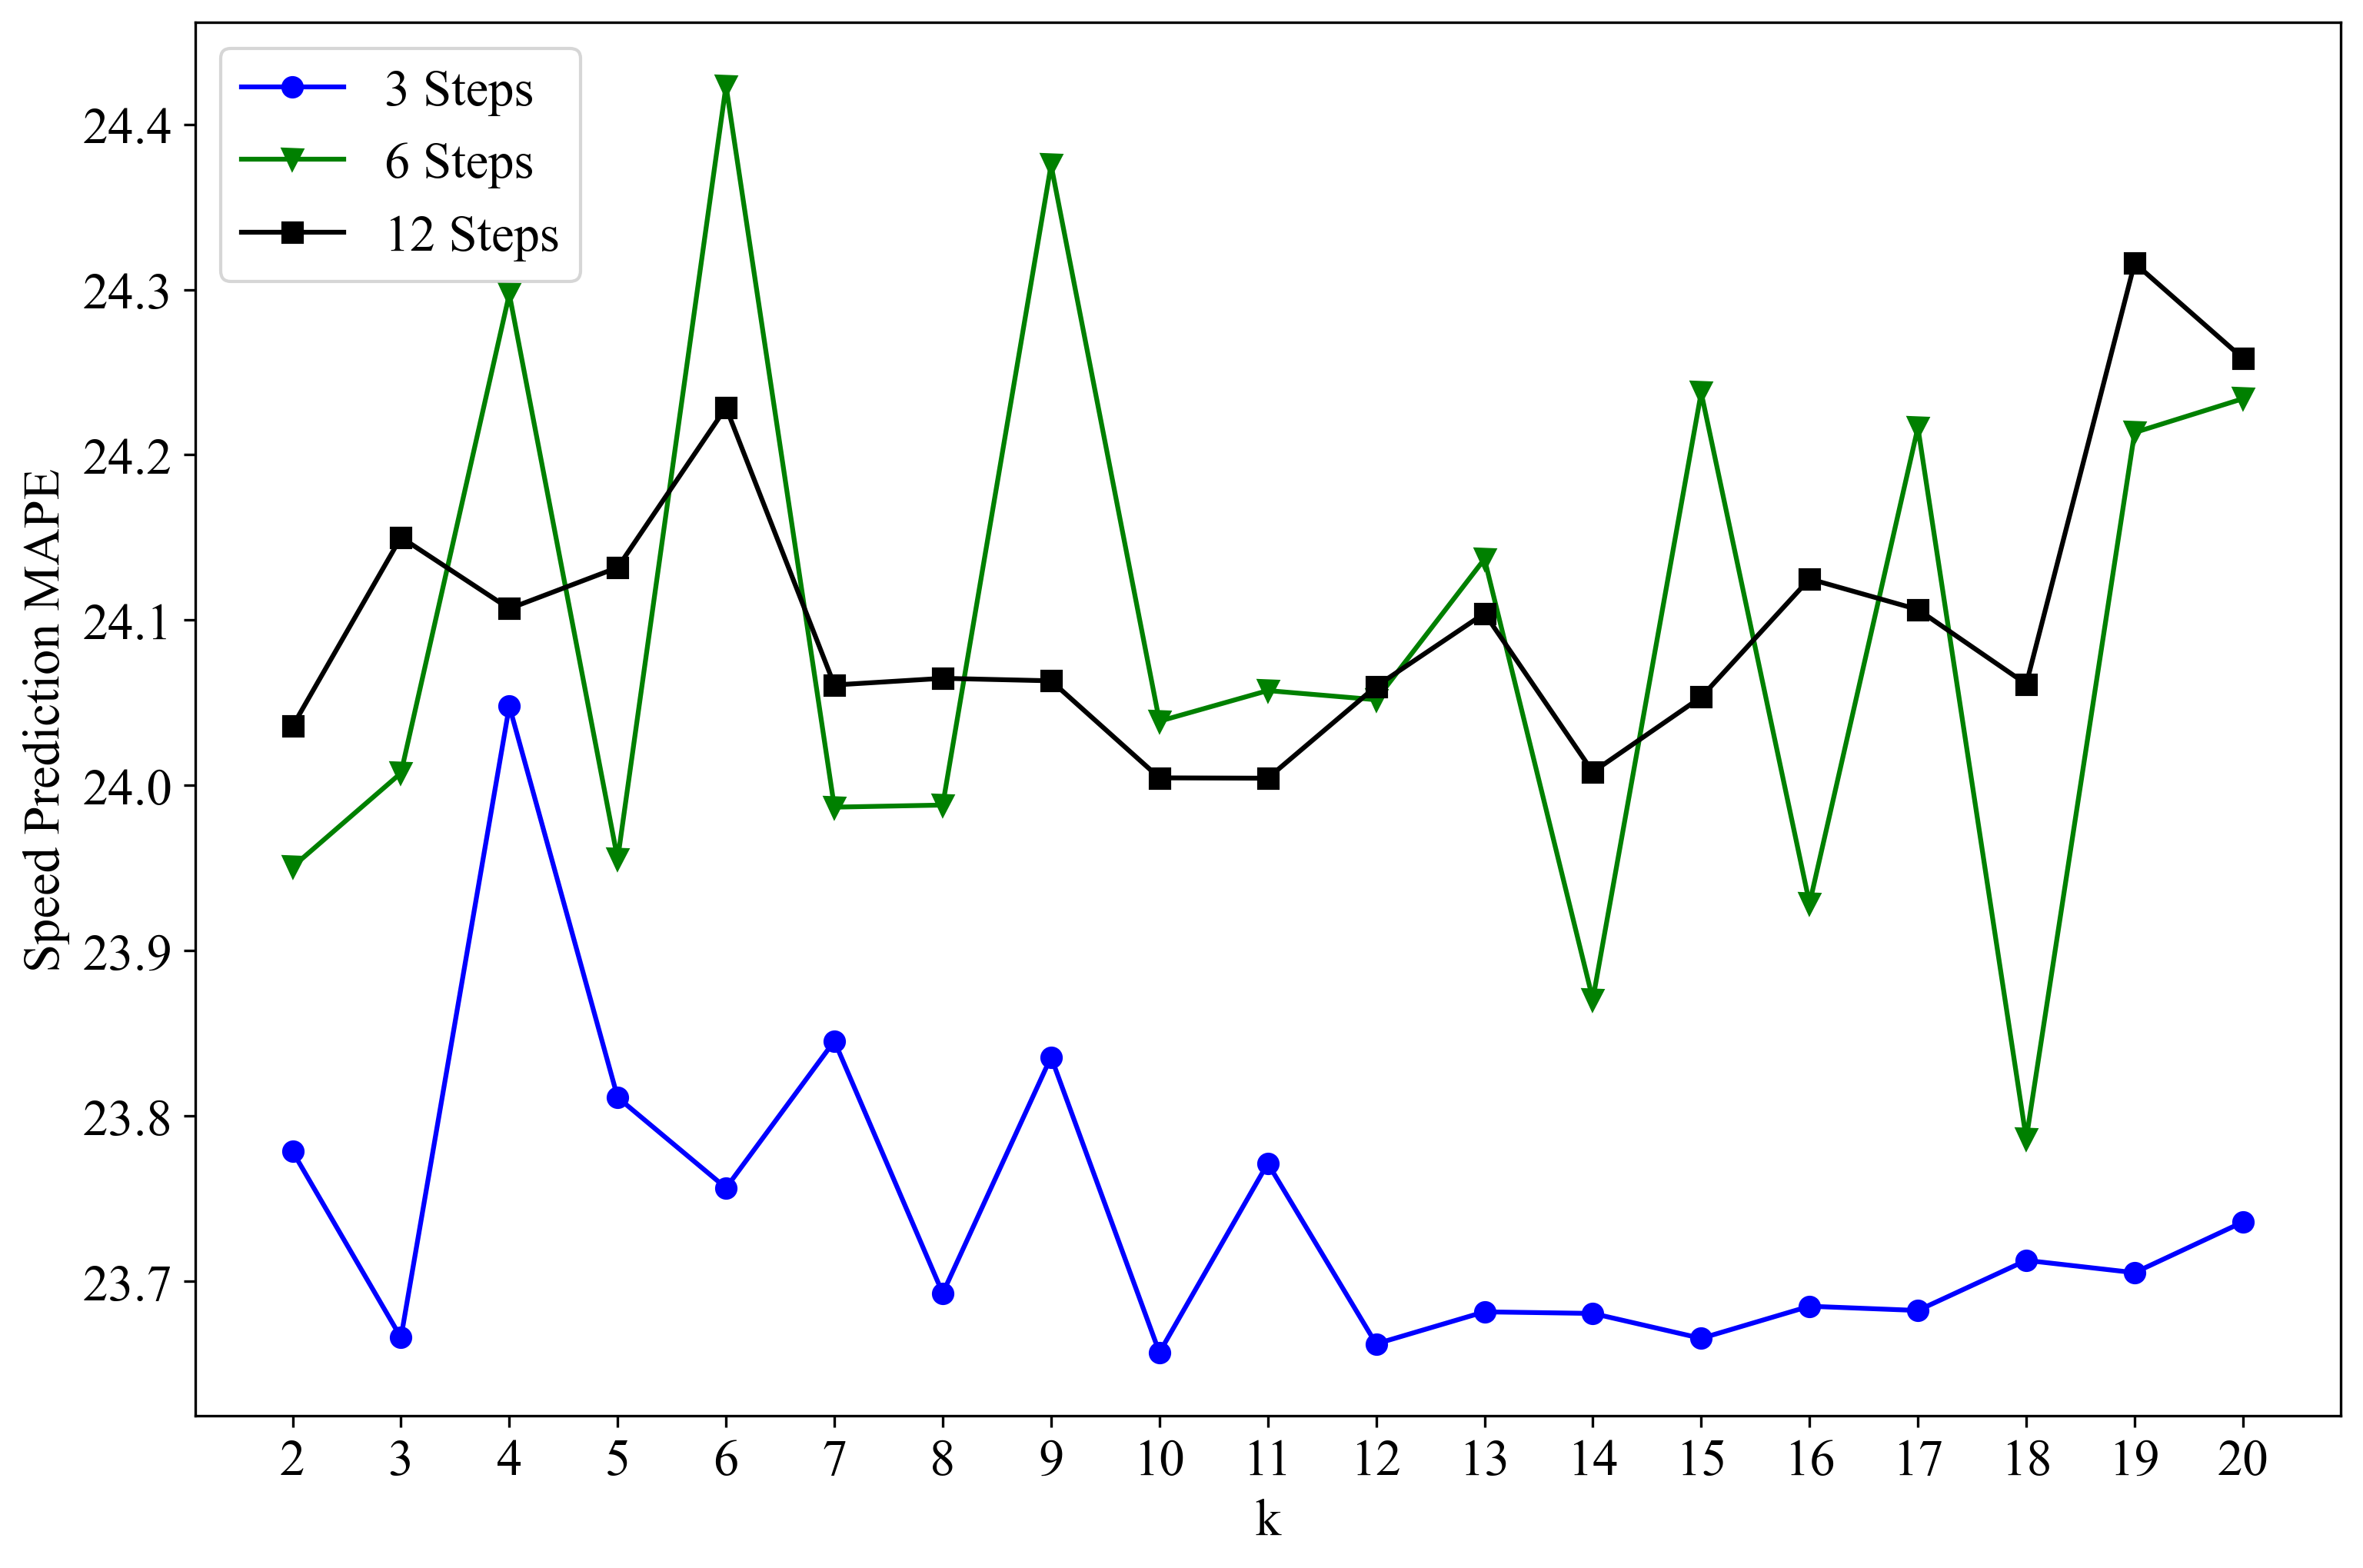
\includegraphics[width=\textwidth]{images/k-speed.png}
        \caption{Traffic speed prediction}
        \label{fig: k-speed}
    \end{subfigure}
\end{figure}
Secondly, we analyze the choice of $k$ when calculating \textit{refined adjacency matrix} $A'$. As shown in figure \ref{fig: k}, the prediction \textit{MAPE} changes randomly with the increase of $k$ from $2$ to $20$. Because the value in $A'$ is either zero or one, a small change can lead to totally different results. There is no general rule for us to determine the value of $k$. Therefore, according to the figure, we choose different $k$ for each step's prediction, which are given in table \ref{k_table}.
\begin{table}[htb]
    \renewcommand\arraystretch{1.5} % 1.5 line space
    \begin{center}
        \caption{The choices of $k$ for $A'$ generation.}
        \label{k_table}
        \begin{tabular}{c|c|c}
            \toprule
  
            \textbf{Model} & \textbf{Traffic State} & \textbf{$k$}\\
  
            \hline
  
            \multirow{2}{*}{STGCN-$A'$} & Flow & $19$\\
            \cline{2-3}
            ~ & Speed & $10$\\

            \hline

            \multirow{2}{*}{DCRNN-$A'$} & Flow & $8$\\
            \cline{2-3}
            ~ & Speed & $10$\\

            \hline

            \multirow{2}{*}{GWNET-$A'$} & Flow & $6$\\
            \cline{2-3}
            ~ & Speed & $11$\\
  
            \bottomrule
        \end{tabular}
    \end{center}
\end{table}

\subsection{Road Correlation Case Study}
In this section, we give a visualization for road correlation and select a specific road for a case study. At first, figure \ref{fig: heatmap} provides the heatmap of road correlations among $r_{225}$ to $r_{245}$. We selected these roads due to the space limitation. In the figure, the correlation values are normalized by MinMax normalization algorithm, and shown as a color block in the heatmap. Some rows have more high-value blocks compared to others. For example, row 241 and row 242. It indicates that some roads have high correlations with most roads in the road network. Referring to figure \ref{fig: gps_seq} and figure \ref{fig: road_correlation_map}, it can be seen that $r_{241}$ and $r_{242}$ are main roads of this district, which confirms our observation.

\begin{figure}[htb]
    \centering
    \caption{Visualization of road correlations.}
    \label{fig: vis_road_cor}
    \begin{subfigure}[t]{0.33\linewidth}
        \centering
        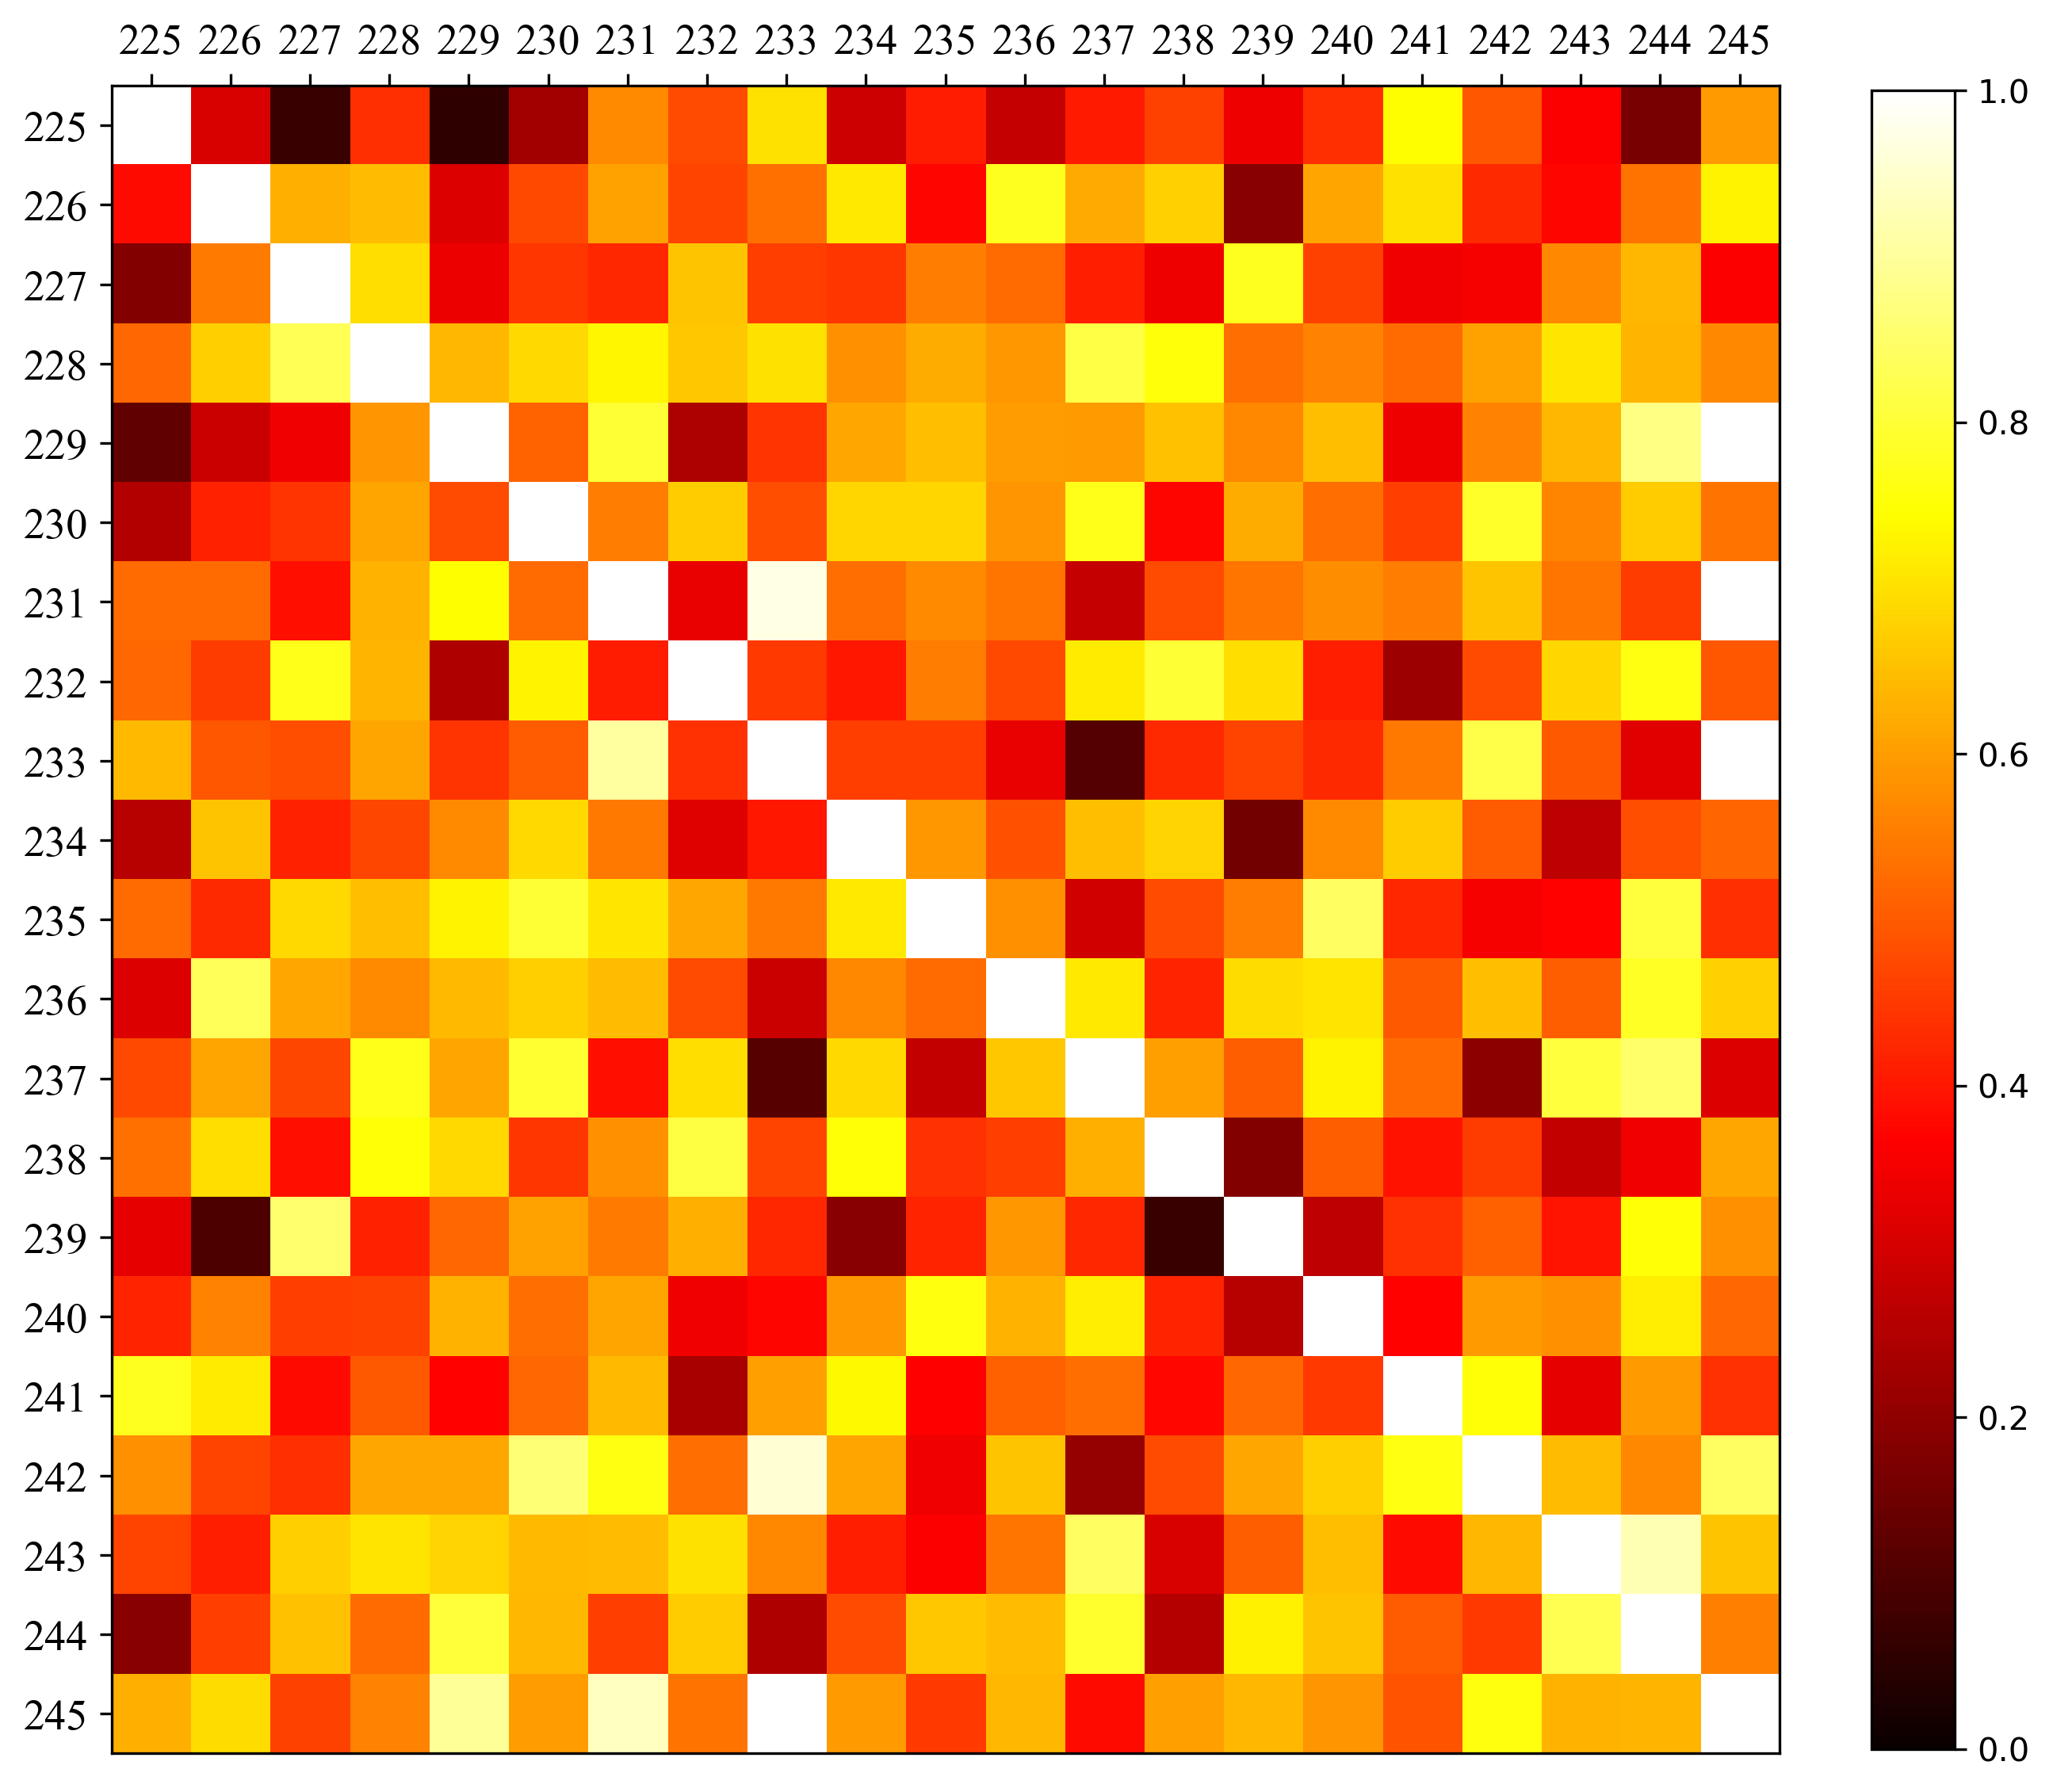
\includegraphics[width=\textwidth]{images/heatmap.png}
        \caption{Heatmap}
        \label{fig: heatmap}
    \end{subfigure}
    \begin{subfigure}[t]{0.66\linewidth}
        \centering
        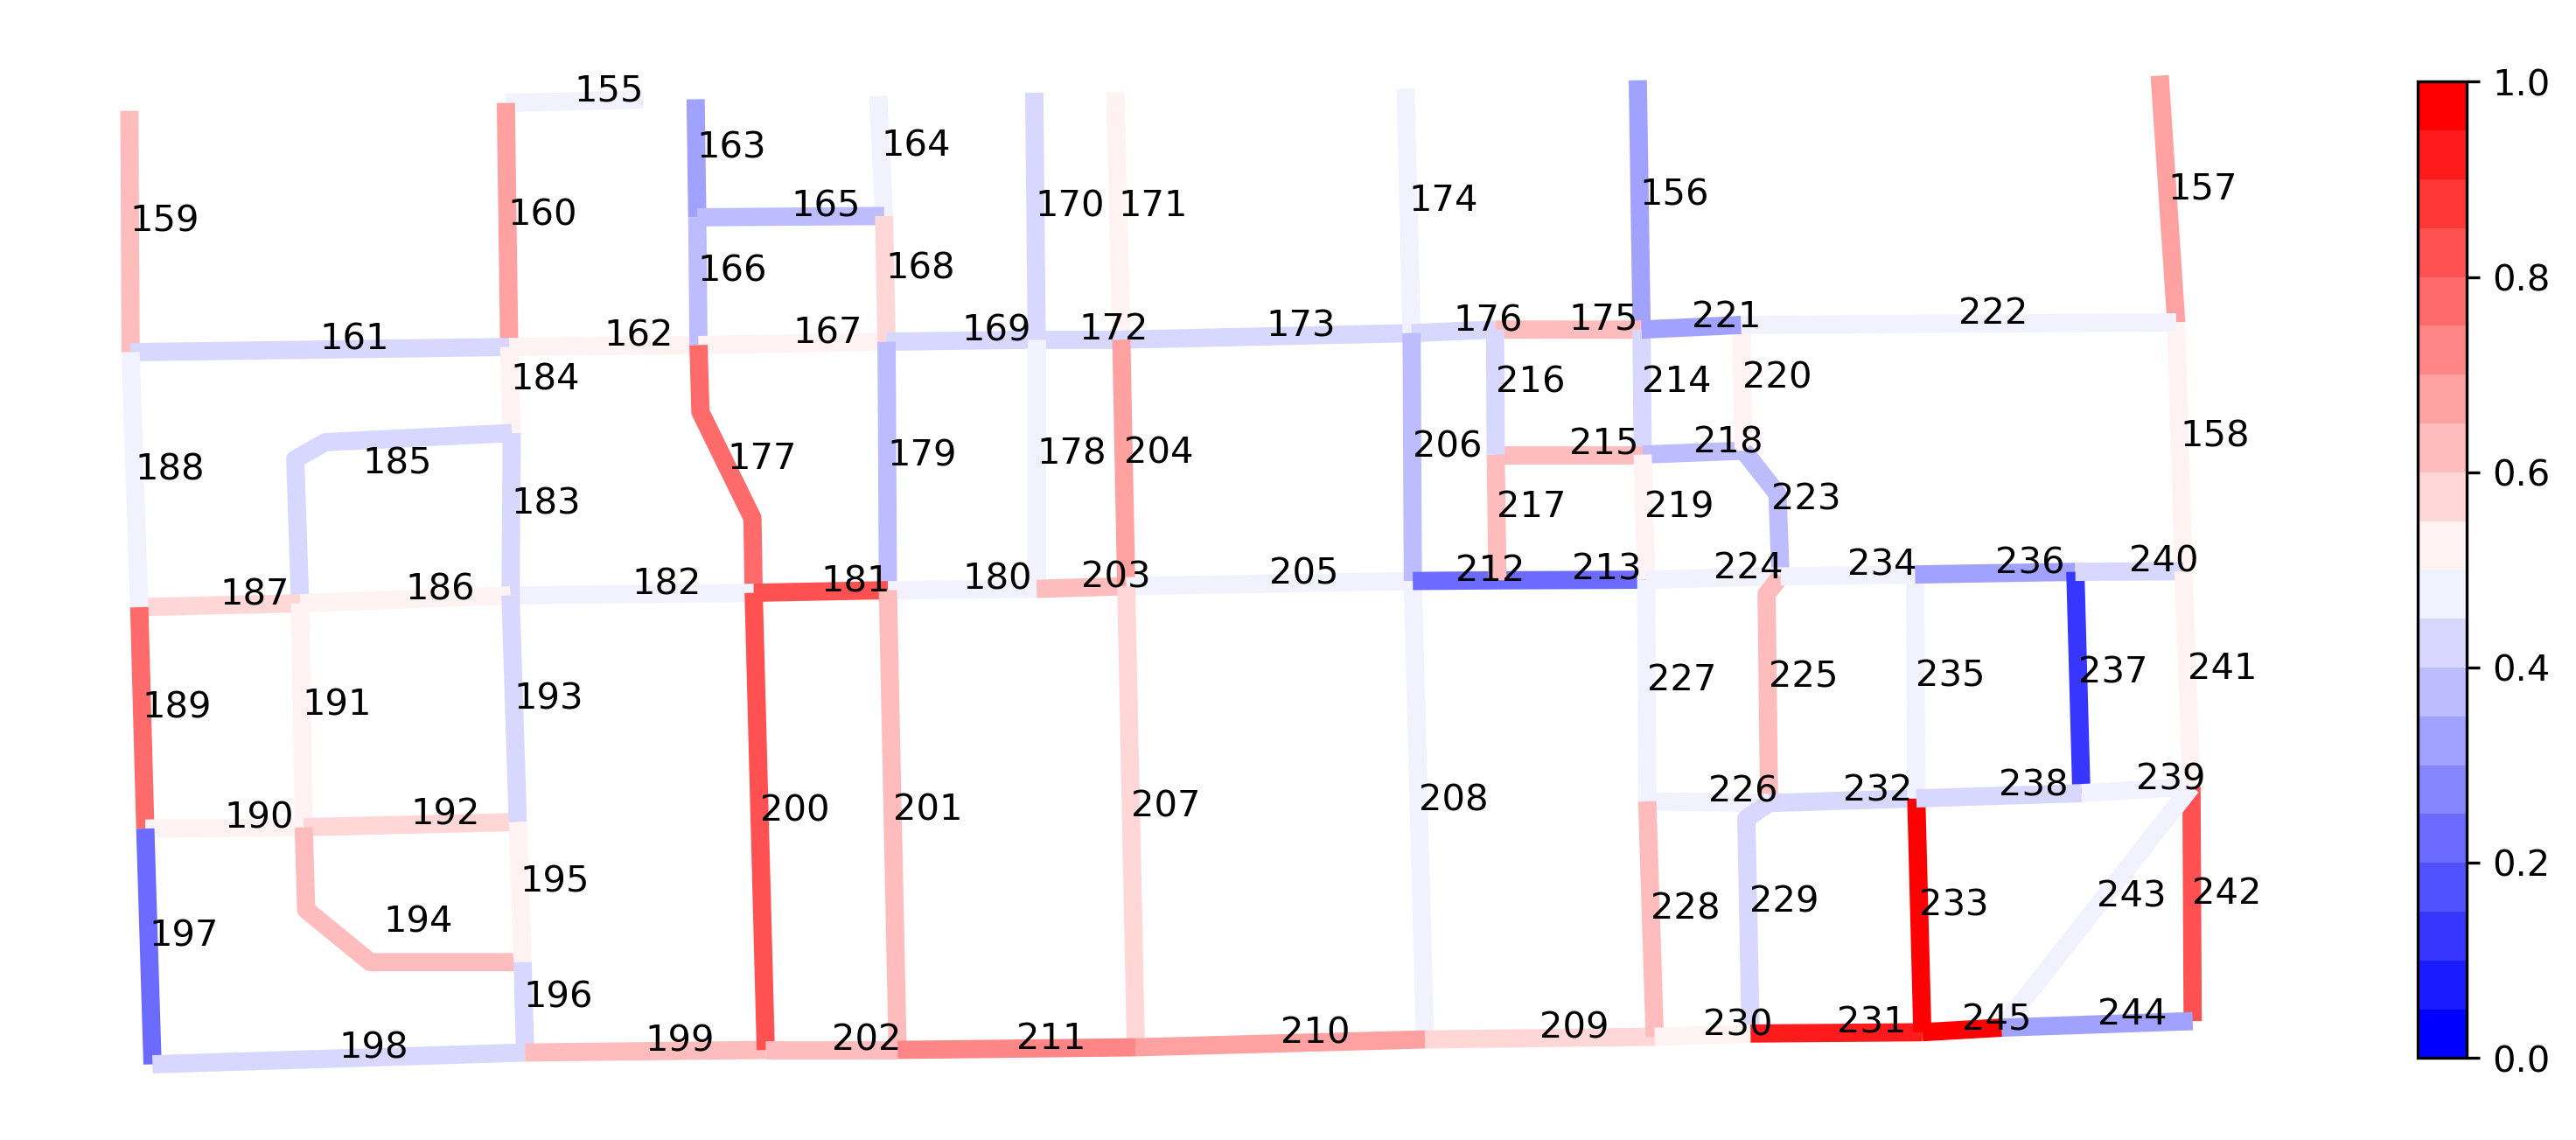
\includegraphics[width=\textwidth]{images/road_correlation.png}
        \caption{Road correlations of $r_{233}$ on map}
        \label{fig: road_correlation_map}
    \end{subfigure}
\end{figure}

% \begin{figure}[htb]
%     \centering
%     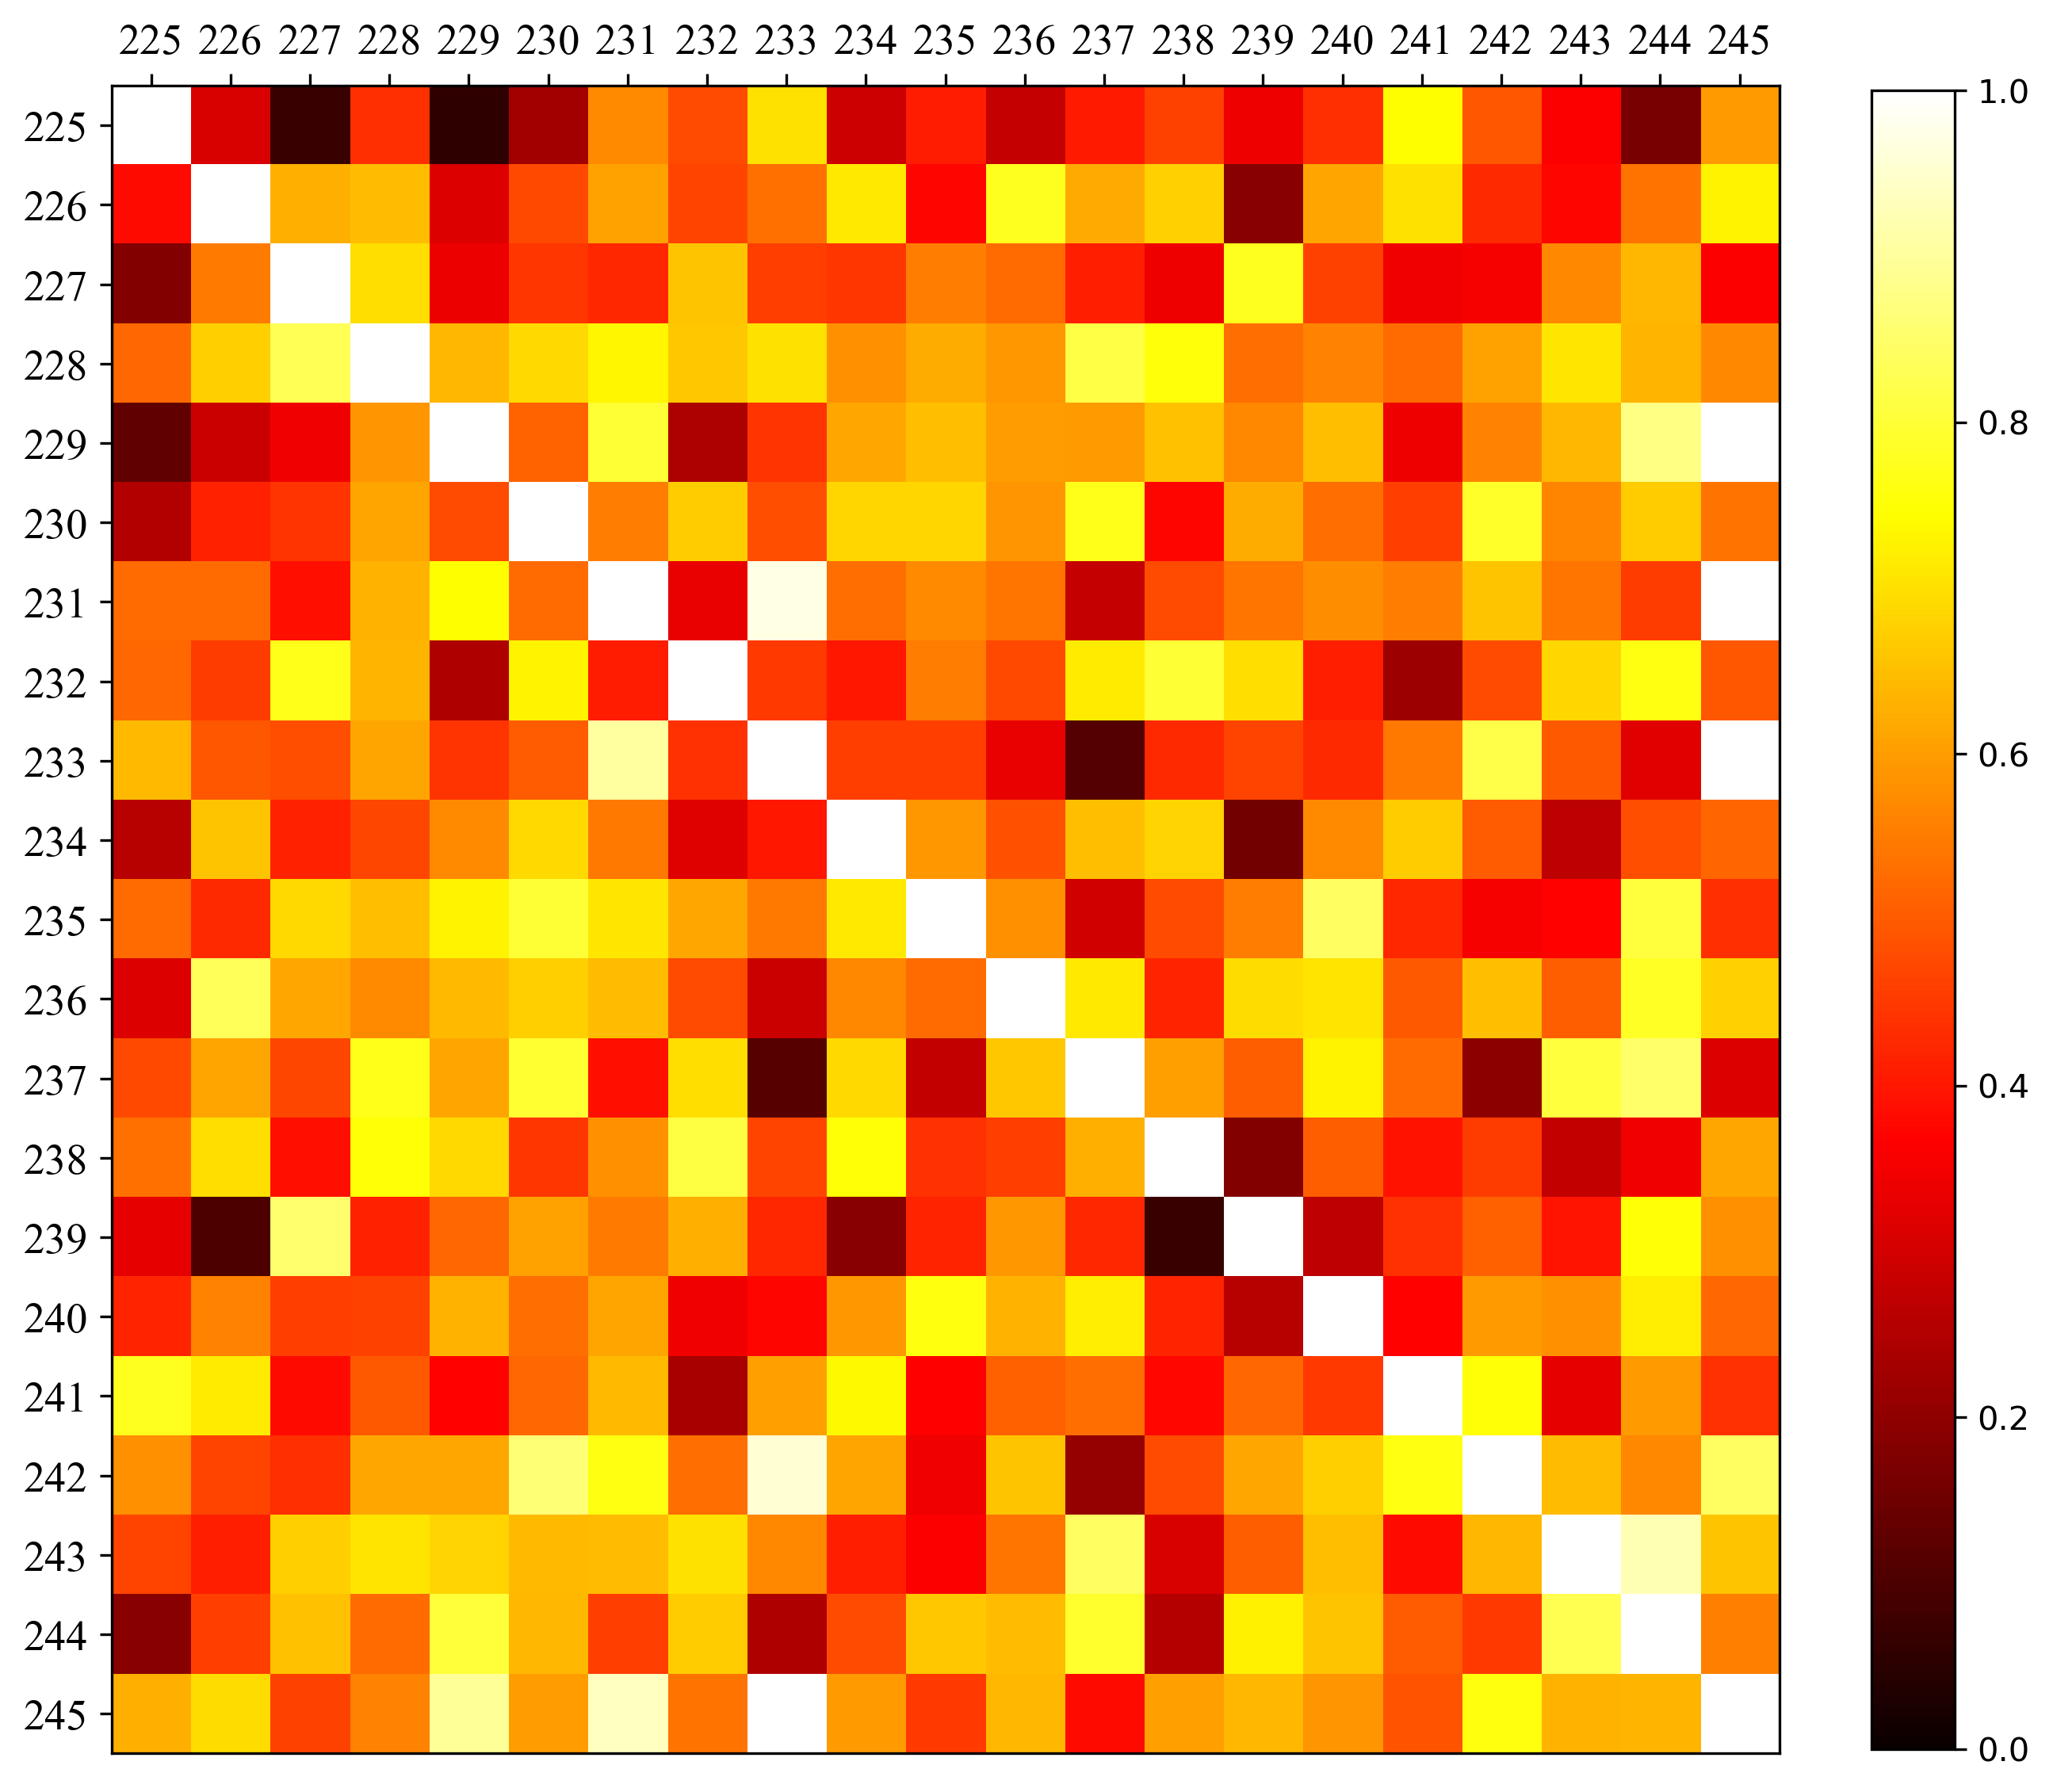
\includegraphics[width=\textwidth]{images/heatmap.png}
%     \caption{Road correlations heatmap.}
%     \label{fig: heatmap}
% \end{figure}

For the visualization on road network, we select roads $r_{155}$ to $r_{245}$, in total 91 roads, which lie in the bottom half of the road network, to visualize the road correlations among them. The road correlation values are taken directly from \textit{road correlation matrix} $C$, which is also the same as the row 233 in the heatmap. As a result, the figure \ref{fig: road_correlation_map} shows the correlations of road $r_{233}$ with other roads. The red road in the bottom right corner stands for $r_{233}$, while other roads are drawn by the color bar according to their correlation values. A redder color means that the corresponding road has a higher correlation with $r_{233}$, and vice versa. If a road is pure blue in the figure, then it has no correlation with $r_{233}$ at all. From the figure, we can observe that the nearby roads, which are $r_{231}, r_{245}, r_{242}, \dots$, are highly correlated with $r_{233}$. It meets our expectation because according to the map, they are $r_{233}$'s upstream and downstream roads, which means our model successfully captured the low-order dependencies. What's more, some long distance roads, such as $r_{200}, r_{181}, r_{177}$, also have considerable correlations with $r_{233}$, which are the high-order dependencies captured by the model. In short, the figure proves that the low and high-order spatial dependencies are both captured by our next-hop prediction model.

% \begin{figure}[htb]
%     \centering
%     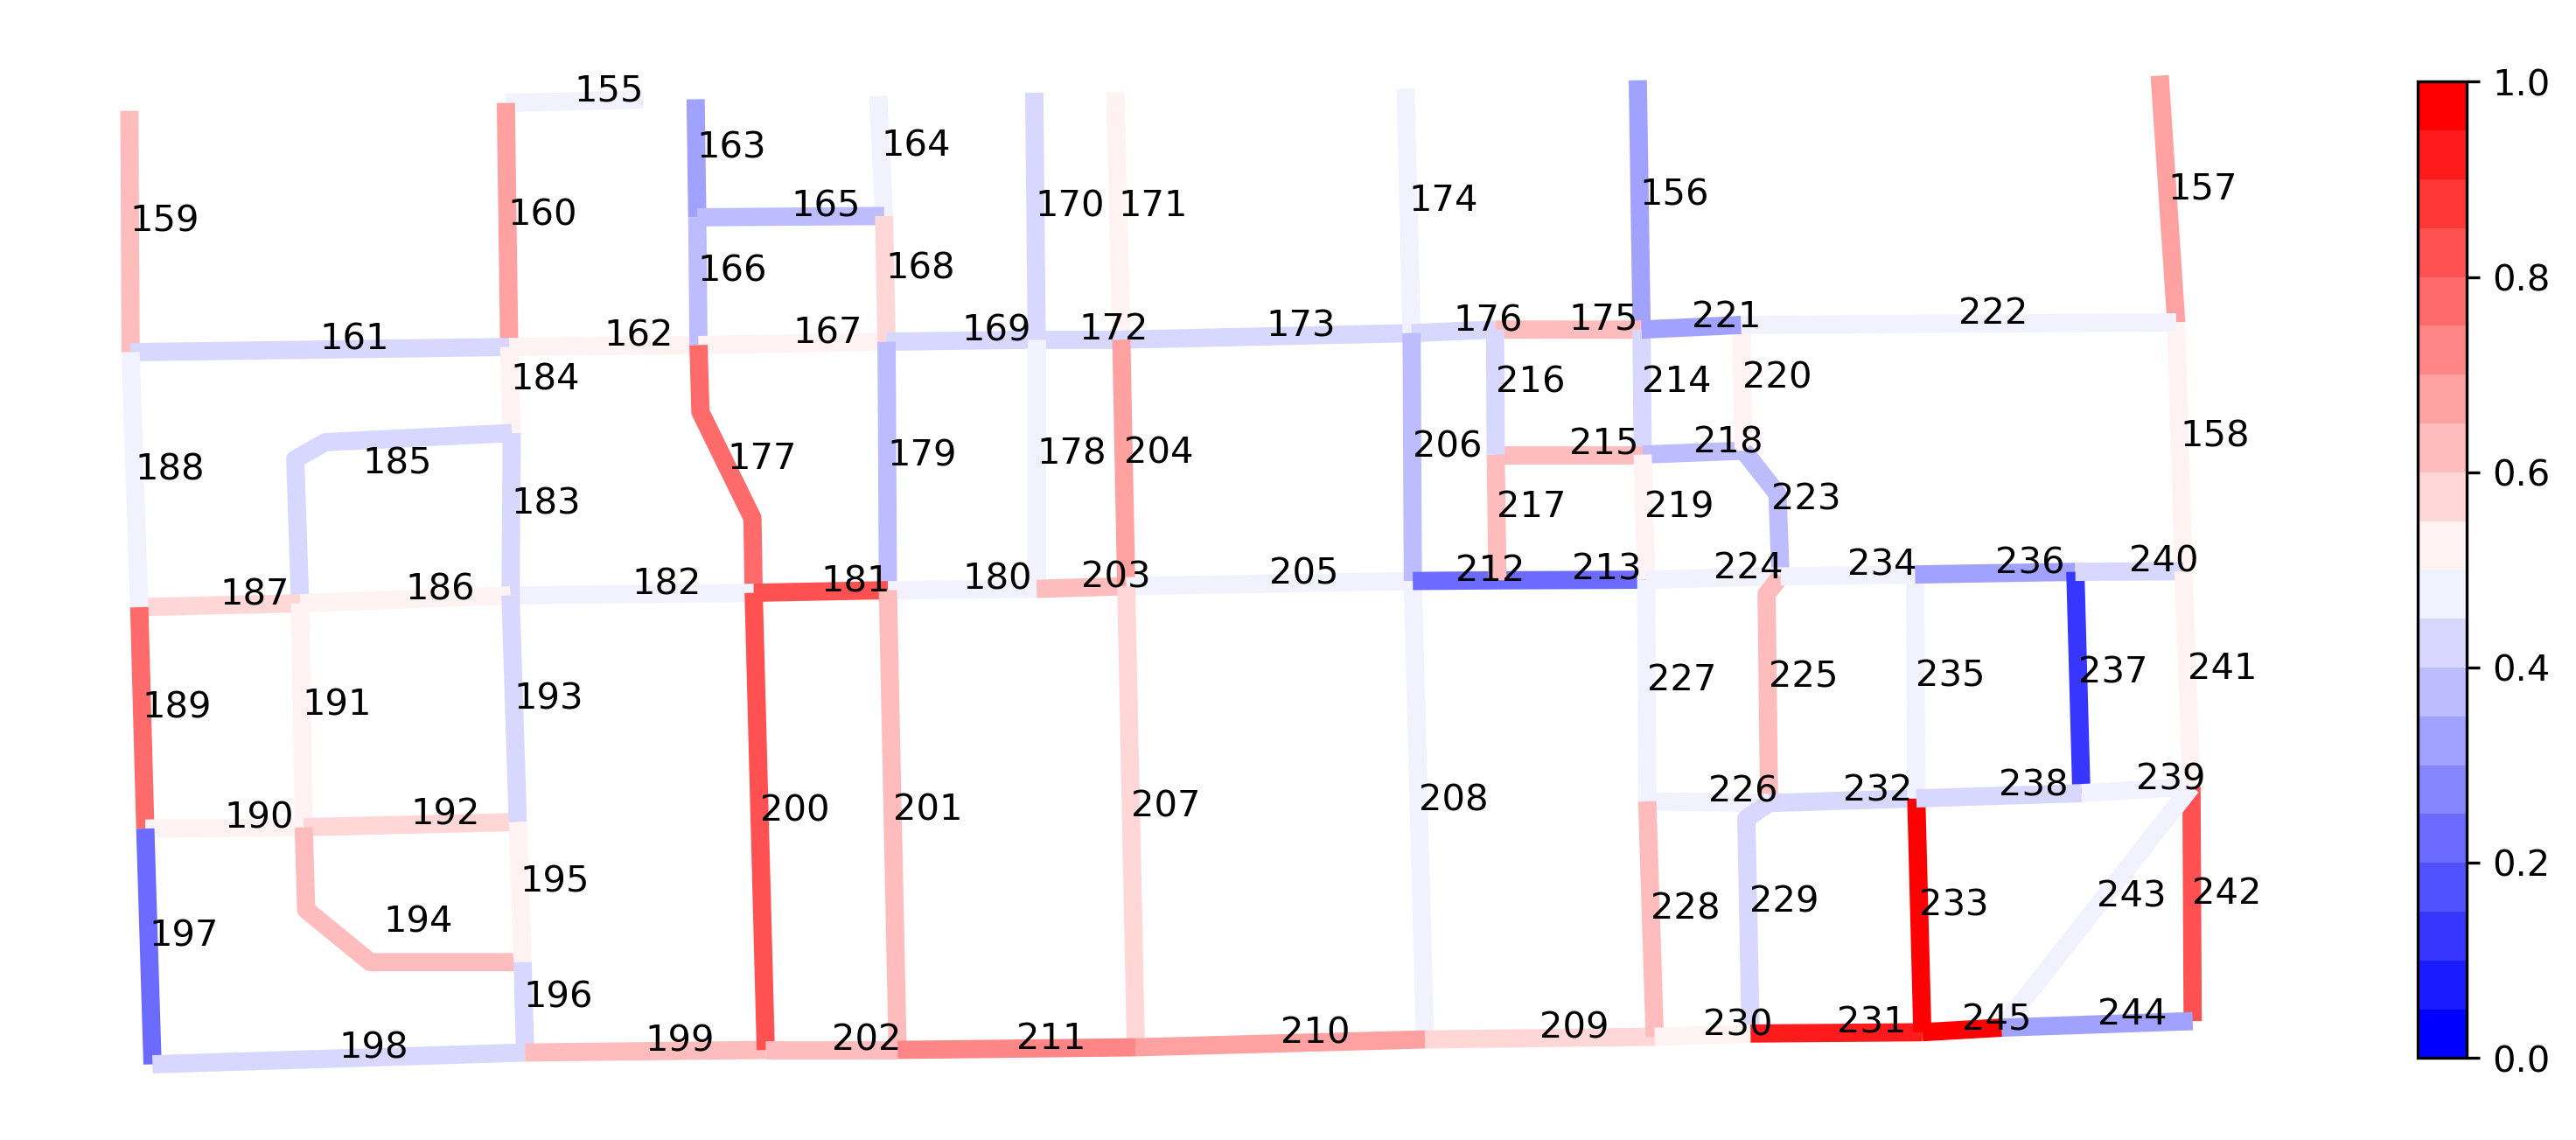
\includegraphics[width=\textwidth]{images/road_correlation.png}
%     \caption{Visualization for road correlations of $r_{233}$.}
%     \label{fig: road_correlation_map}
% \end{figure}

\begin{figure}[htb]
    \centering
    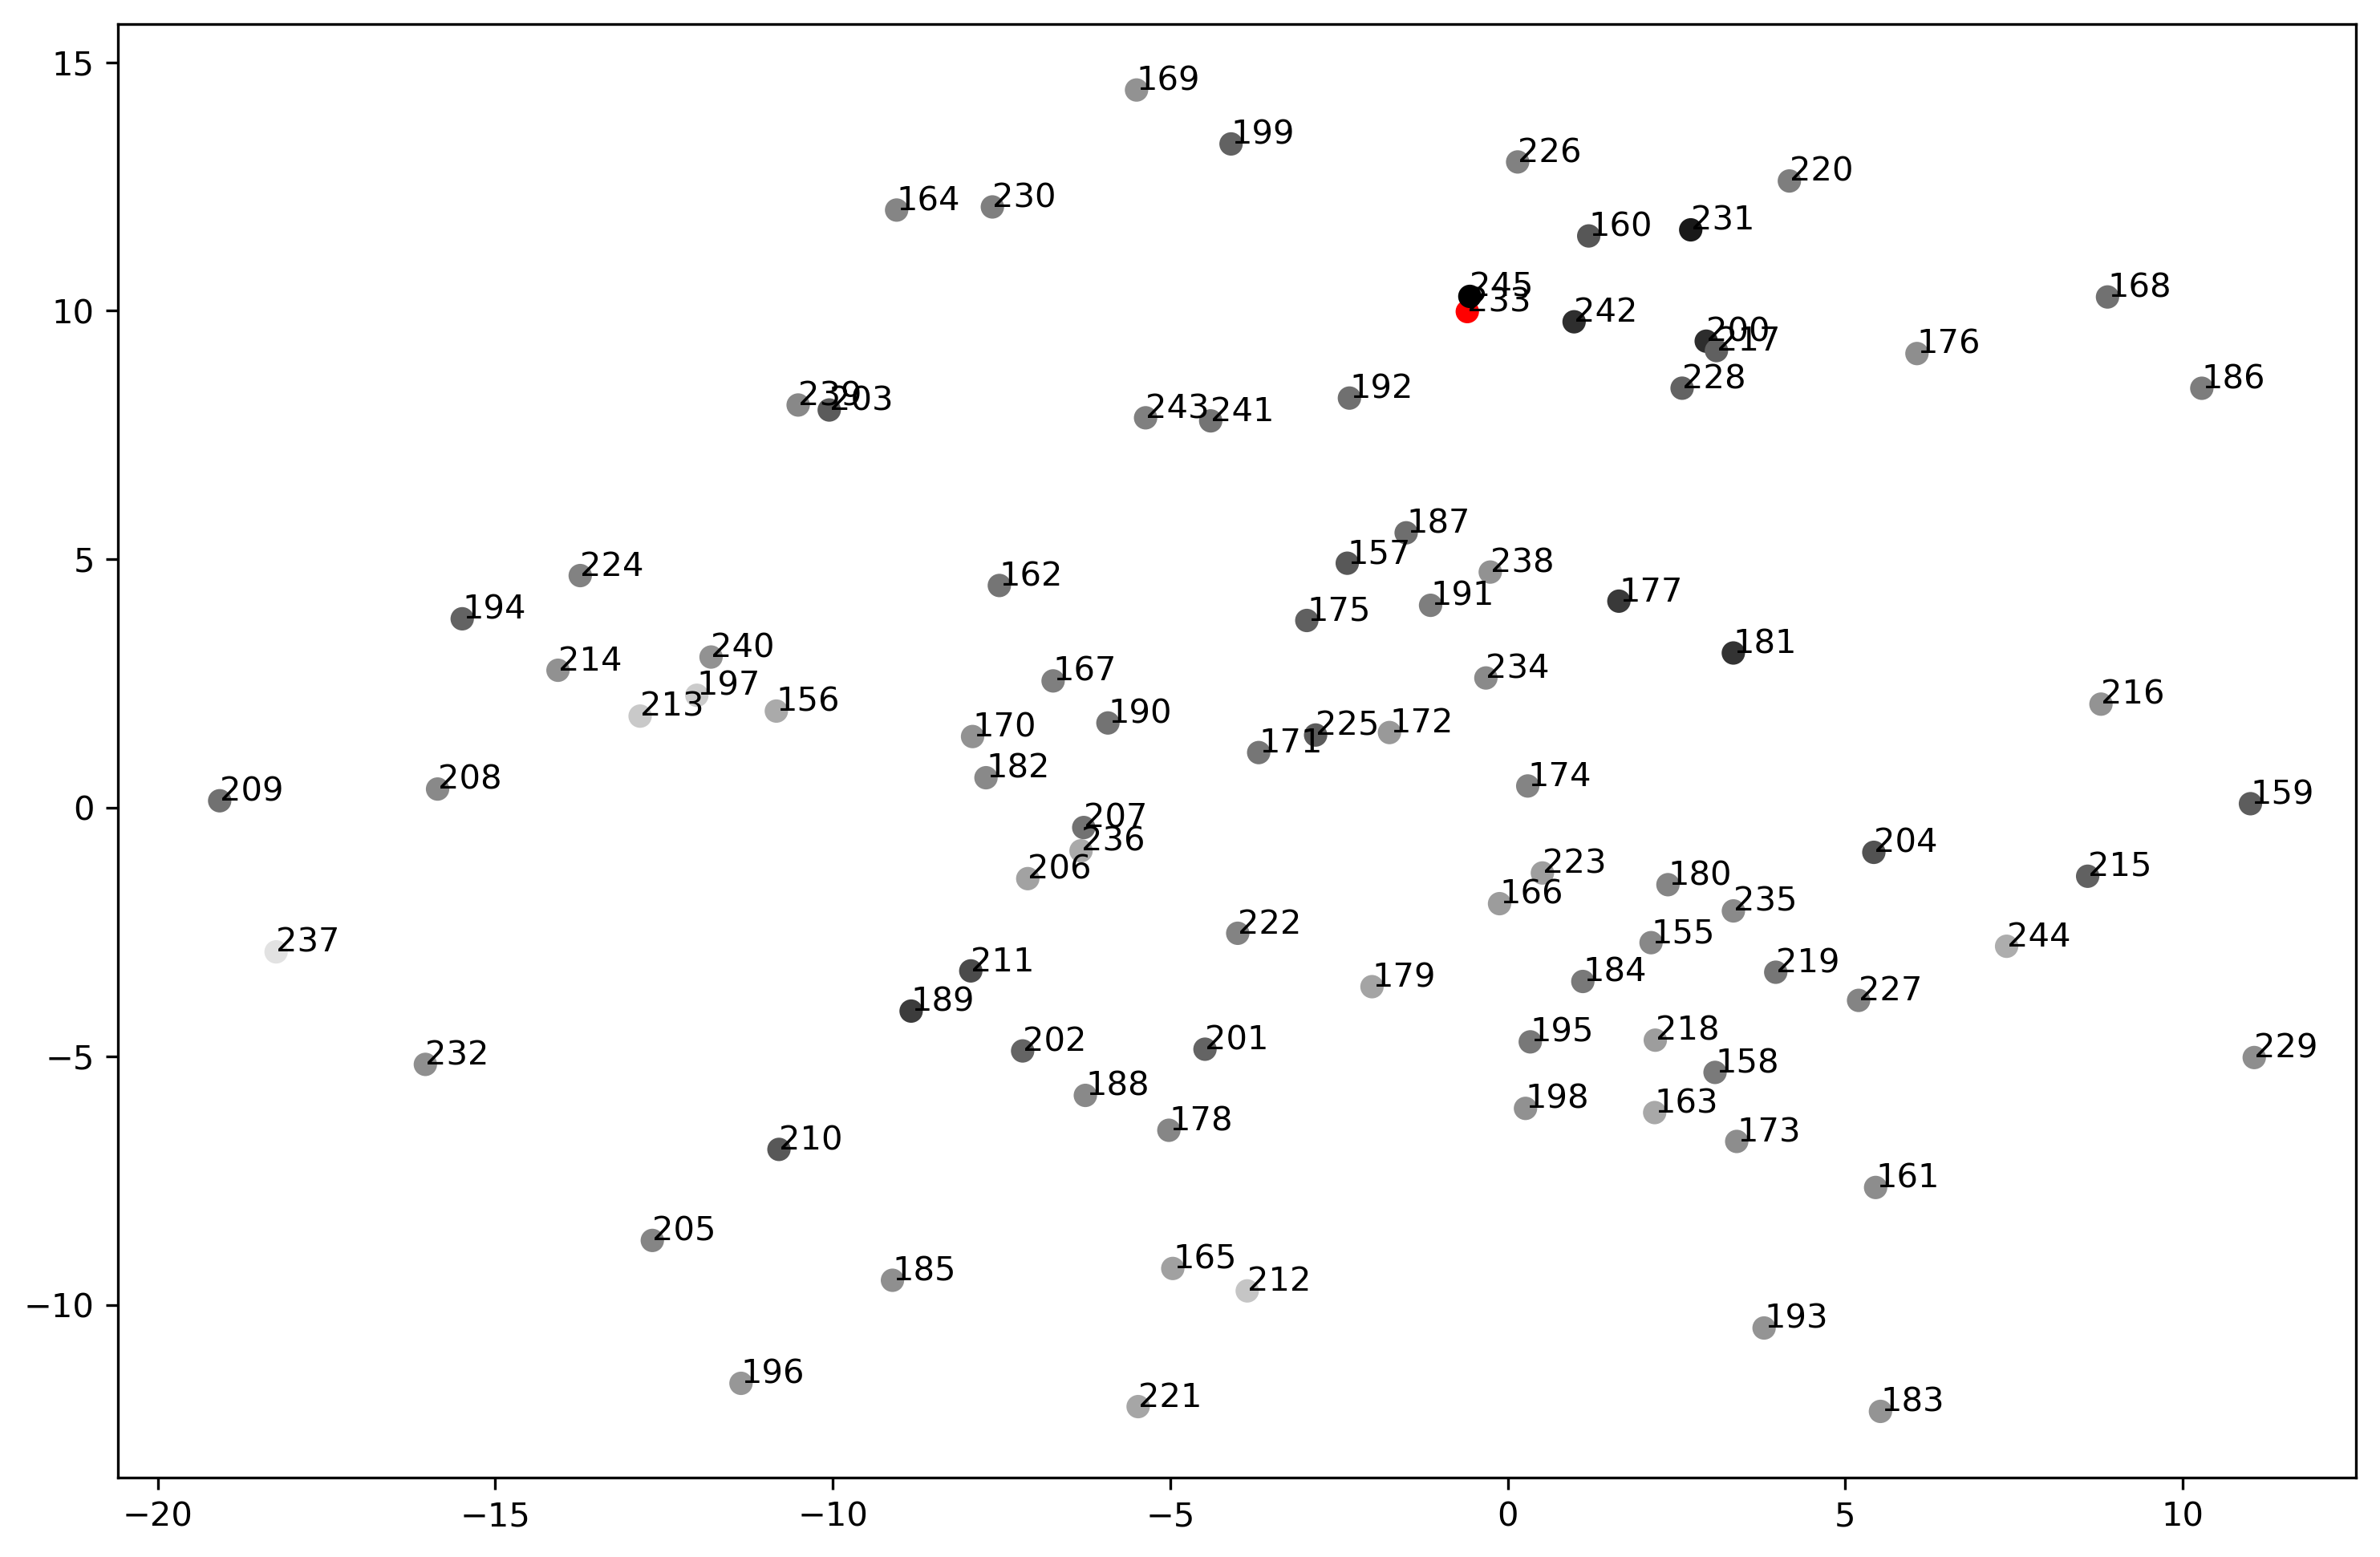
\includegraphics[width=\textwidth]{images/road_tsne.png}
    \caption{Road embedding points after t-SNE dimensionality reduction.}
    \label{fig: road_correlation_tsne}
\end{figure}

Next, starting from road embedding matrix $E$, we perform t-SNE\cite{tsne} algorithm to reduce the embedding dimension from $d_r=64$ to $2$, and plot the points on a 2-D figure. The color of each road remains same as figure \ref{fig: road_correlation_map}, where the red point still stands for $r_{233}$. If $C$ is able to represent the road correlations, then the high-correlated roads mentioned above should be close to the red point. As shown in figure \ref{fig: road_correlation_tsne}, the points for $r_{245}, r_{242}, r_{231}, r_{200}, r_{177}, r_{181}$ are near to $r_{233}$, which means $C$ is able to represent the similarity between road embedding vectors, i.e. road correlation.

In conclusion, these two case experiments prove not only the rationality of our thesis on \textit{trajectory-based road correlation}, but also the effectiveness of our proposed model and methods.
